\documentclass{beamer}

\mode<presentation>
{
	\usepackage{StyleFiles/Rome}
	\setbeamercovered{transparent}
}

\mode<handout>
{
	\usepackage{pgfpages}
	\pgfpagesuselayout{2 on 1}[a4paper,border shrink=5mm]
	\nofiles
}

\usepackage[english]{babel}
\usepackage[algoruled]{algorithm2e}
\usepackage{movie15}
\usepackage{rotating}
\usepackage{subfigure}
\usepackage{dsfont}

\definecolor{darkgreen}{RGB}{0,180,0}
\definecolor{lightred}{RGB}{210,0,0}

\setbeamertemplate{itemize subitem}{\tiny\raise1.5pt\hbox{\donotcoloroutermaths$ \blacktriangleright $}}

\title[Predicting Future Agent Motions through a Distributed Multi-Clustered PF]{\Large Predicting Future Agent Motions through a Distributed Multi- Clustered Particle Filtering}

\subtitle{}

\author[Fabio Previtali]{\Large\textbf{Fabio Previtali}}

\date[May 9, 2016]{Learning in Autonomous Systems\\A.Y. 2015/2016\\Rome, Italy}

\begin{document}

\begin{frame}[plain]
	\titlepage
\end{frame}

\section{Introduction to Distributed Data Fusion}

\begin{frame}
	\frametitle{Multi-Agent Multi-Object Tracking (MAMOT)}
	\framesubtitle{A brief overview}
	
	\begin{columns}
		\column{.7\textwidth}
		\centering
		
		\begin{block}{Object Tracking}
			Detect objects and follow their trajectories
		\end{block}
		
		\begin{block}{MAMOT}
			A team of agents estimate the object trajectories using sensors with a limited field-of-view
		\end{block}
		
		\begin{itemize}
			\item distributed environment (network connected agents)
			\item best-effort communication channel
		\end{itemize}
		
		\column{.28\textwidth}
		\centering
		
		\begin{tikzpicture}
			\node at (0,0) [draw=black,ultra thick,inner sep=0pt]  {\includegraphics[width=3cm]{Figures/Player.png}};
		\end{tikzpicture}
	\end{columns}
\end{frame}

\begin{frame}
	\frametitle{Issues on DDF}
	\framesubtitle{The Data Association problem}
	
	\begin{columns}[T]
		\column{.55\textwidth}
		
		\begin{itemize}
			\only<1>{\item In MAMOT, the pool of gathered parameters are used to compute the global estimation}
			\only<1>{\item Using a Particle Filter, one of the main problem that arises is how to avoid poor estimation
						   quality}
			\only<1>{\vspace{3.42cm}}
			\only<2->{\item The weight of particles is evaluated using the received parameters}
			\only<3->{\vspace{1.5cm}\item[1] Using all parameters influences the whole distribution}
			\only<4-5>{\vspace{1.1cm}}
			\only<6>{\vspace{0.9cm}}
			\only<4>{\item[2] We can assign better weights by use clustering before weighting}
			\only<5>{\item[2] The parameters are associated to the clusters}
			\only<6>{\item[2] The weights of particles in a cluster is given by the parameters associated to it}
		\end{itemize}
		
		\column{.45\textwidth}
		\centering
		
		\begin{tikzpicture}
			\only<1>
			{
				\node at (0,0) [draw=white,thick,inner sep=0pt]  {\includegraphics[width=5cm]{Figures/MamotDDF.pdf}};
			}
			\only<2->
			{
				\node at (-1.3,0) [draw=white,thick,inner sep=0pt]  {\includegraphics[width=2.5cm]{Figures/Issue0.pdf}};
				\node at (1.3,0) [draw=white,thick,inner sep=0pt]  {\includegraphics[width=2.5cm]{Figures/Issue0Bis.pdf}};
				\node at (0,-1) [inner sep=0pt]  {\includegraphics[width=5cm]{Figures/Parentheses.pdf}};
				\node at (0,-2.5) [draw=white,thick,inner sep=0pt]  {\includegraphics[width=4cm]{Figures/IssueBlank.pdf}};
				\node at (0,-4.8) [draw=white,thick,inner sep=0pt]  {\includegraphics[width=4cm]{Figures/IssueBlank.pdf}};
			}
			\only<3->
			{
				\node at (0,-2.5) [draw=white,thick,inner sep=0pt]  {\includegraphics[width=4cm]{Figures/Issue1.pdf}};
				\node at (0,-4.8) [draw=white,thick,inner sep=0pt]  {\includegraphics[width=4cm]{Figures/IssueBlank.pdf}};
			}
			\only<4>
			{
				\node at (0,-4.8) [draw=white,thick,inner sep=0pt]  {\includegraphics[width=4cm]{Figures/Issue2.pdf}};
			}
			\only<5>
			{
				\node at (0,-4.8) [draw=white,thick,inner sep=0pt]  {\includegraphics[width=4cm]{Figures/Issue2Bis.pdf}};
			}
			\only<6>
			{
				\node at (0,-4.8) [draw=white,thick,inner sep=0pt]  {\includegraphics[width=4cm]{Figures/Issue2Ter.pdf}};
			}
		\end{tikzpicture}
	\end{columns}
\end{frame}

\section{Handson}

\begin{frame}
	\frametitle{}
	
	\Huge
	
	\vspace{0.5cm}
	
	\begin{center}
		\textbf{PTracking}
	\end{center}
\end{frame}

\begin{frame}
	\frametitle{Hands-on PTracking}
	\framesubtitle{Getting Library}
	
	\Large
	
	\emph{PTracking} is currently available at the following repo:
	\begin{center}
		\url{https://fabioprev@bitbucket.org/fabioprev/ptracking.git}
	\end{center}
	
	\vspace{0.2cm}
	
	Currently the only supported platform is \textbf{Linux}.
\end{frame}

\begin{frame}
	\frametitle{Hands-on PTracking}
	\framesubtitle{Dependencies}
	
	\Large
	
	On Xubuntu (Ubuntu) 14.04 LTS (kernel 3.13.0-37) and later versions, you need to install
	the following packages:
	
	\vspace{0.2cm}
	
	\begin{columns}[T]
		\column{.5\textwidth}
		
		\begin{itemize}
			\item build-essential
			\item cmake
			\item libxml2
			\item libxml2-dev
			\item libboost1.54-all-dev
		\end{itemize}
		
		\column{.5\textwidth}
		\centering
		
		\begin{itemize}
			\item libopencv-dev
			\item libopenni2-dev (optional)
			\item gnuplot (optional)
			\item gnuplot-x11 (optional)
		\end{itemize}
	\end{columns}
\end{frame}

\begin{frame}
	\frametitle{Hands-on PTracking}
	\framesubtitle{Building Library}
	
	\Large
	
	We recommend a so-called out of source building, which can be achieved by the following command
	sequence:
	
	\vspace{0.2cm}
	
	\begin{itemize}
		\item \texttt{cd <PTracking-root-directory>}
		\item \texttt{mkdir build}
		\item \texttt{cd build}
		\item \texttt{cmake ../src}
		\item \texttt{make -j<number-of-cores+1>}
	\end{itemize}
\end{frame}

\begin{frame}
	\frametitle{Hands-on PTracking}
	\framesubtitle{Installing Library}
	
	\Large
	
	\vspace{0.4cm}
	
	The library can be optionally installed (which we suggest) by typing the following command
	sequence:
	
	\vspace{0.2cm}
	
	\begin{itemize}
		\item \texttt{cd <PTracking-root-directory>/build}
		\item \texttt{sudo make install}
	\end{itemize}
	
	\vspace{0.3cm}
	
	\textbf{Header files:} \texttt{/usr/local/include/PTracking} \\
	
	\vspace{0.1cm}
	
	\textbf{Shared objects:} \texttt{/usr/local/lib/PTracking} \\
	
	\vspace{0.1cm}
	
	\textbf{Binaries:} \texttt{/usr/local/bin} \\
	
	\vspace{0.5cm}
	
	\textbf{Warning:} First logout before starting using the library
\end{frame}

\begin{frame}
	\frametitle{Hands-on PTracking}
	\framesubtitle{Running Library}
	
	\Large
	
	
\end{frame}

\begin{frame}
	\frametitle{Projects}
	
	\LARGE
	
	\begin{block}{Project \# 1}
		Study \textbf{how} the tracking parameters - for example the \emph{closenessThreshold} -
		\textbf{influence} the data association process. The analyse should accurately report the
		\textbf{variation} - in terms of MOTA and MOTP - of the performance while \textbf{varying} the
		tracking parameters.
	\end{block}
\end{frame}

\begin{frame}
	\frametitle{Projects}
	
	\LARGE
	
	\begin{block}{Project \# 2}
		Study \textbf{how} the sensor calibration \textbf{influences} the tracking performance. The
		analyse should accurately report the \textbf{variation} - in terms of MOTA and MOTP - of the
		performance while \textbf{varying} the precision in the calibration phase.
	\end{block}
\end{frame}

\section{Related Work - Tracking}

\begin{frame}
	\frametitle{Related Work}
	\framesubtitle{Multi-object tracking}
	
	\Large
	
	\vspace{0.6cm}
	
	Multi-object tracking algorithms can be classified into two groups (Andriyenko \emph{et al.}
	\cite{Andriyenko11}):
	
	\begin{itemize}
		\item \textbf{Global} (or \emph{offline}): formulating the tracking problem as an optimisation
			  one, where all the trajectories within a temporal window are optimised jointly
		\item \textbf{Recursive} (or \emph{online}): estimating the current state relying only on the
			  current observations and on the previous state
	\end{itemize}
	
	\vspace{0.45cm}
	
	\tiny
	
	[1] A. Andriyenko \emph{et al.}, ``An analytical formulation of global occlusion reasoning for
		multi target tracking'', ICCV, 2011
\end{frame}

\begin{frame}
	\frametitle{Multi-Object Tracking}
	\framesubtitle{Global methods}
	
	\Large
	
	\vspace{0.2cm}
	
	\begin{itemize}
		\item \textbf{Berclaz} \emph{et al.} \cite{Berclaz11}: mathematically sound
			  multiple object tracking framework based on a k-shortest path optimization
			  algorithm
		\vspace{0.1cm}
		\item \textbf{Leal-Taix{\'e}} \emph{et al.} \cite{Leal11}: formulate a new graph
			  model for the multiple object tracking challenge by minimizing a network flow
			  problem
		\vspace{0.1cm}
		\item \textbf{Henriques} \emph{et al.} \cite{Henriques11}: 
		\vspace{0.1cm}
		\item ...
	\end{itemize}
\end{frame}

\begin{frame}
	\frametitle{Multi-Object Tracking}
	\framesubtitle{Recursive methods}
	
	\Large
	
	\vspace{0.2cm}
	
	\begin{itemize}
		\item \textbf{Breitenstein} \emph{et al.} \cite{Breitenstein11}: online method for
			  multi-person tracking-by-detection in a particle filtering framework
		\vspace{0.1cm}
		\item \textbf{Yang} \emph{et al.} \cite{Yang09}: probabilistic appearance model
			  method for tracking multiple people
		\vspace{0.1cm}
		\item \textbf{Bae} \emph{et al.} \cite{Bae14}: 
		\vspace{0.1cm}
		\item ...
	\end{itemize}
\end{frame}

\begin{frame}
	\frametitle{Global vs Recursive Methods}
	
	\Large
	
	\begin{table}[!t]
		\centering
		\begin{tabular}{ c | c | c | }
			\cline{2-3}
			& \textbf{Global} & \textbf{Recursive} \\ \hline
			
			\multicolumn{1}{|c|}{\textbf{Accuracy}} & medium/high & medium/high \\ \hline
			\multicolumn{1}{|c|}{\textbf{Precision}} & \textbf{high} & medium/high \\ \hline
			\multicolumn{1}{|c|}{\textbf{Robustness}} & \textbf{high} & medium/high \\ \hline
			\multicolumn{1}{|c|}{\textbf{Computational Load}} & high & \textbf{low}/medium \\ \hline
			\multicolumn{1}{|c|}{\textbf{Real-time}} & no & \textbf{yes}/no \\ \hline
		\end{tabular}
	\end{table}
	
	Global methods are more precise and robust but they cannot be used in real systems:
	\begin{itemize}
		\item No information from the future are available
		\item Frame rate not suitable for real-time applications
	\end{itemize}
\end{frame}

\section{PTracking}

\begin{frame}
	\frametitle{PTracking}
	
	\vspace{0.15cm}
	
	\begin{columns}[T]
		\column{.53\textwidth}
		
		\vspace{0.8cm}
		
		\begin{itemize}
			\item \textbf{Input:} a set of positions of the objects provided by a multi
				  object detection system
			
			\vspace{1.6cm}
			
			\item \textbf{Output:} a set of estimated trajectories of the moving objects
				  over time
		\end{itemize}
		
		\column{.5\textwidth}
		\centering
		
		\begin{tikzpicture}
			\node at (0,0) [draw=black,ultra thick,inner sep=0pt]
			{
				\includegraphics[width=5.8cm]{Figures/Detection}
			};
			\node at (0,-3.35) [draw=black,ultra thick,inner sep=0pt]
			{
				\includegraphics[width=5.8cm]{Figures/Tracking}
			};
		\end{tikzpicture}
	\end{columns}
\end{frame}

\begin{frame}
	\frametitle{PTracking}
	\framesubtitle{Pseudo-code}
	
	\begin{columns}[T]
		\column{.05\textwidth}
		
		\column{.55\textwidth}
		
		\only<1>
		{
			\begin{algorithm}[H]
				\tiny
				\KwIn{perceptions $ z_{s,t} $, local track numbers $ i_{s,t-1} $, global track numbers $ I_{s,t-1} $}
				\BlankLine
				\KwData{set of local particles $ \tilde{\xi}_{s,t} $, set of global particles $ \tilde{\xi}_{\mathcal{S'},t} $, local GMM set $ \mathcal{L} $, global GMM set $ \mathcal{G} $}
				\BlankLine
				\KwOut{global estimations $ x_{s,t} = (\boldsymbol{I}_{s,t},\boldsymbol\Lambda_{s,t},\boldsymbol{M}_{s,t},\boldsymbol\Sigma_{s,t}) $}
				\BlankLine
				\Begin
				{
					\textcolor{darkgreen}{$ \tilde{\xi}_{s,t} \sim \pi_t (x_{s,t} | x_{s,t-1},z_{s,t}) $}
					\BlankLine
					\textcolor{darkgreen}{Re-sample by using the SIR principle}\\
					\BlankLine
					\textcolor{darkgreen}{$ \mathcal{L} = KClusterize(\tilde{\xi}_{s,t}) $}
					\BlankLine
					\textcolor{darkgreen}{$ (\boldsymbol{i}_{s,t},\boldsymbol\lambda_{s,t},\boldsymbol\mu_{s,t},\boldsymbol\sigma_{s,t}) = DataAssociation(\mathcal{L}, i_{s,t-1}) $}
					\BlankLine
					\textcolor{darkgreen}{Communicate belief $ (\boldsymbol{i}_{s,t},\boldsymbol\lambda_{s,t},\boldsymbol\mu_{s,t},\boldsymbol\sigma_{s,t}) $ to other agents}
				}
				\BlankLine
				\Begin
				{
					Collect $ \mathcal{L}_{S'} $ from a subset $ \mathcal{S'} \subseteq \mathcal{S} $ of sensors within a $ \Delta t $
					\BlankLine
					$ \tilde{\xi}_{\mathcal{S'},t} \sim \tilde\pi = \sum_{s \in \mathcal{S'}} \boldsymbol\lambda_{s,t} \, \mathcal{N} (\boldsymbol\mu_{s,t},\boldsymbol\sigma_{s,t}) $
					\BlankLine
					Re-sample by using the SIR principle\\
					\BlankLine
					$ \mathcal{G} = KClusterize(\tilde\xi_{{\mathcal{S'},t}}) $
					\BlankLine
					$ (\boldsymbol{I}_{s,t},\boldsymbol\Lambda_{s,t},\boldsymbol{M}_{s,t},\boldsymbol\Sigma_{s,t}) = DataAssociation(\mathcal{G},I_{s,t-1}) $
				}
			\end{algorithm}
			
			\column{.01\textwidth}
			
			\Huge
			\vspace{2.15cm}
			
			\begin{center}
				\textcolor{blue}{$ \Rightarrow $}
			\end{center}
			
			\column{.44\textwidth}
			
			\centering
			
			\begin{tikzpicture}
				\node at (0,0) [draw=black,ultra thick,inner sep=0pt]
				{
					\includegraphics[width=3.3cm]{Figures/Mamot-1}
				};
				\node at (0,-3.5) [draw=black,ultra thick,inner sep=0pt]
				{
					\includegraphics[width=3.3cm]{Figures/Mamot-2}
				};
			\end{tikzpicture}
		}
		
		\only<2->
		{
			\begin{algorithm}[H]
				\tiny
				\KwIn{perceptions $ z_{s,t} $, local track numbers $ i_{s,t-1} $, global track numbers $ I_{s,t-1} $}
				\BlankLine
				\KwData{set of local particles $ \tilde{\xi}_{s,t} $, set of global particles $ \tilde{\xi}_{\mathcal{S'},t} $, local GMM set $ \mathcal{L} $, global GMM set $ \mathcal{G} $}
				\BlankLine
				\KwOut{global estimations $ x_{s,t} = (\boldsymbol{I}_{s,t},\boldsymbol\Lambda_{s,t},\boldsymbol{M}_{s,t},\boldsymbol\Sigma_{s,t}) $}
				\BlankLine
				\Begin
				{
					$ \tilde{\xi}_{s,t} \sim \pi_t (x_{s,t} | x_{s,t-1},z_{s,t}) $
					\BlankLine
					Re-sample by using the SIR principle\\
					\BlankLine
					$ \mathcal{L} = KClusterize(\tilde{\xi}_{s,t}) $
					\BlankLine
					$ (\boldsymbol{i}_{s,t},\boldsymbol\lambda_{s,t},\boldsymbol\mu_{s,t},\boldsymbol\sigma_{s,t}) = DataAssociation(\mathcal{L}, i_{s,t-1}) $
					\BlankLine
					Communicate belief $ (\boldsymbol{i}_{s,t},\boldsymbol\lambda_{s,t},\boldsymbol\mu_{s,t},\boldsymbol\sigma_{s,t}) $ to other agents
				}
				\BlankLine
				\Begin
				{
					\textcolor{lightred}{Collect $ \mathcal{L}_{S'} $ from a subset $ \mathcal{S'} \subseteq \mathcal{S} $ of sensors within a $ \Delta t $}
					\BlankLine
					\textcolor{lightred}{$ \tilde{\xi}_{\mathcal{S'},t} \sim \tilde\pi = \sum_{s \in \mathcal{S'}} \boldsymbol\lambda_{s,t} \, \mathcal{N} (\boldsymbol\mu_{s,t},\boldsymbol\sigma_{s,t}) $}
					\BlankLine
					\textcolor{lightred}{Re-sample by using the SIR principle}\\
					\BlankLine
					\textcolor{lightred}{$ \mathcal{G} = KClusterize(\tilde\xi_{{\mathcal{S'},t}}) $}
					\BlankLine
					\textcolor{lightred}{$ (\boldsymbol{I}_{s,t},\boldsymbol\Lambda_{s,t},\boldsymbol{M}_{s,t},\boldsymbol\Sigma_{s,t}) = DataAssociation(\mathcal{G},I_{s,t-1}) $}
				}
			\end{algorithm}
			
			\column{.01\textwidth}
			
			\Huge
			\vspace{2.15cm}
			
			\begin{center}
				\textcolor{blue}{$ \Rightarrow $}
			\end{center}
			
			\column{.44\textwidth}
			
			\centering
			
			\begin{tikzpicture}
				\node at (0,0) [draw=black,ultra thick,inner sep=0pt]
				{
					\includegraphics[width=3.3cm]{Figures/Mamot-1}
				};
				\node at (0,-3.5) [draw=black,ultra thick,inner sep=0pt]
				{
					\includegraphics[width=3.3cm]{Figures/Mamot-3}
				};
			\end{tikzpicture}
		}
	\end{columns}
\end{frame}

\section{Experimental Evaluation - Tracking}

\logo{\includegraphics[height=1cm]{ThemeFigs/Sapienza}\vspace{200pt}}

\begin{frame}
	\frametitle{Evaluating a Tracking Algorithm}
	
	\Large
	
	\vspace{0.45cm}
	
	The CLEAR MOT (Kasturi et al. \cite{Kasturi09}) metrics \emph{MOTA} and \emph{MOTP} are the
	de-facto standard for evaluating a tracking method:
	
	\vspace{-0.5cm}
	
	\begin{equation*}
		MOTA = 1 - \frac{\sum_{t=1}^{N_{frames}} \big [ c_m(m_t) + c_f(fp_t) + cs(ID\mbox{-}S_t) \big ]}{\sum_{t=1}^{N_{frames}} N_G^{(t)}}
	\end{equation*}
	
	\vspace{0.4cm}
	
	\begin{equation*}
		MOTP = \frac{\sum_{i=1}^{N_{mapped}} \sum_{t=1}^{N_{frames}^{(t)}} \Big [ \frac{| G_i^{(t)} \cap D_i^{(t)} |}{| G_i^{(t)} \cup D_i^{(t)} |} \Big ] }{\sum_{t=1}^{N_{frames}} N_{mapped}^{(t)}}
	\end{equation*}
	
	\vspace{0.3cm}
	
	\tiny
	
	\cite{Kasturi09} R. Kasturi \emph{et al.},  ``Framework for performance evaluation of face, text,
	and vehicle detection and tracking in video: data,\\ \hspace{0.25cm} metrics, and protocol'', PAMI,
	2009 \\
\end{frame}

\begin{frame}
	\frametitle{Experimental Evaluation}
	\framesubtitle{Multi-Sensor, Single-Object}
	
	\vspace{-0.1cm}
	
	\begin{center}
		\begin{tikzpicture}
			\node at (-4.2,0) [draw=black,ultra thick,inner sep=0pt]
			{
				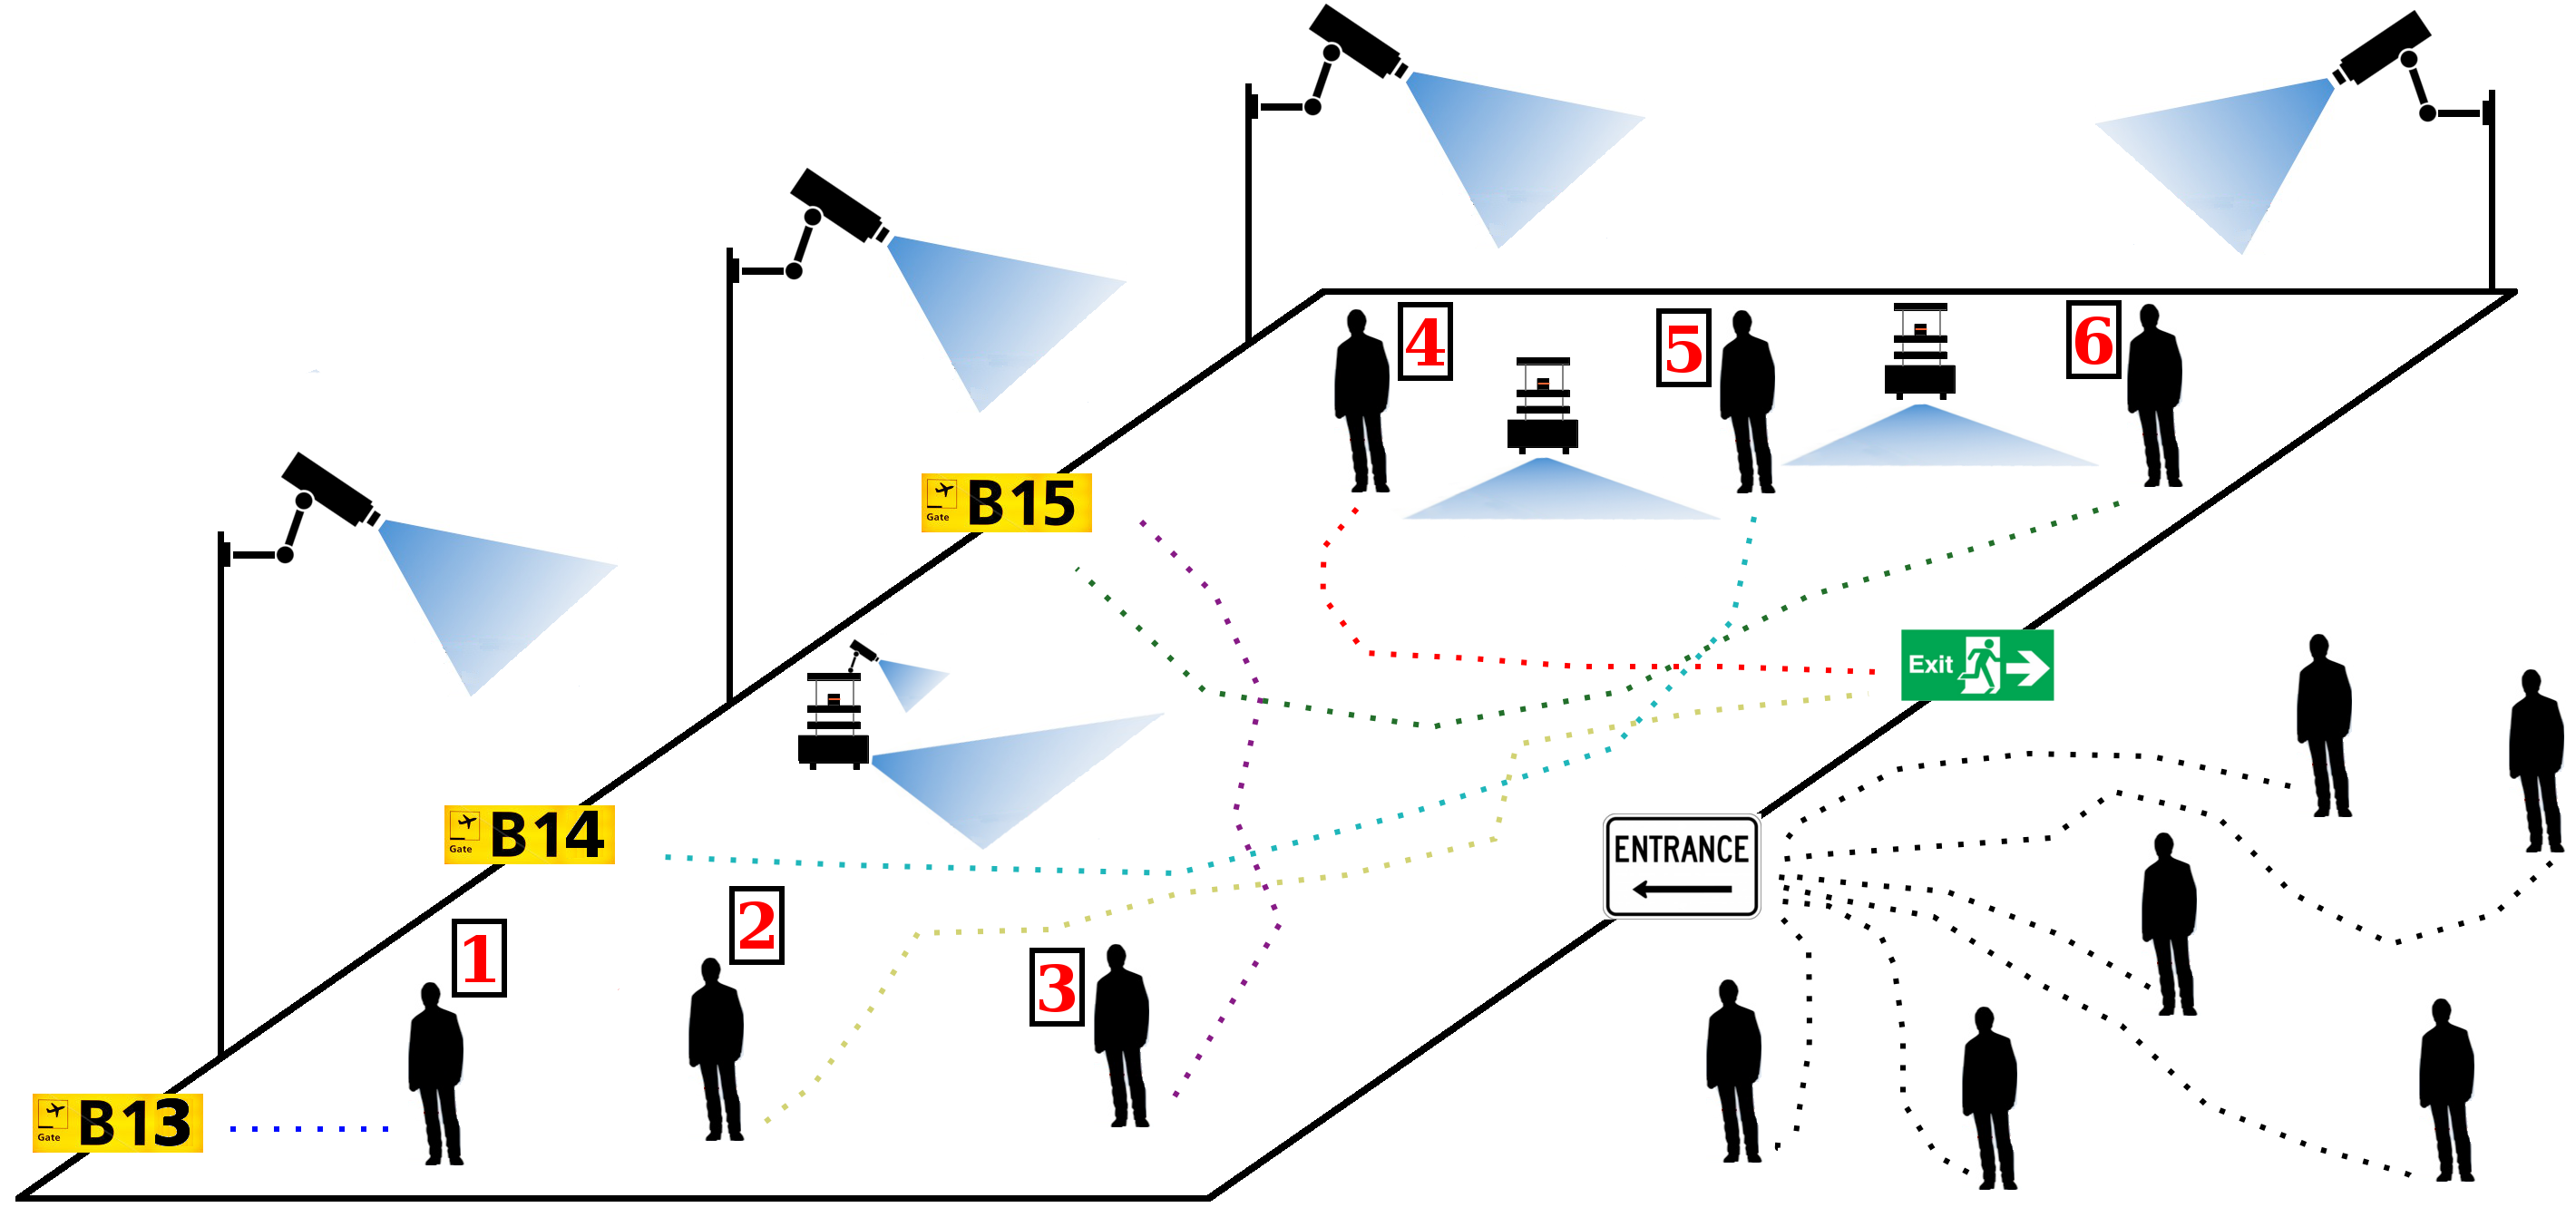
\includegraphics[scale=0.125]{Figures/Challenge}
			};
			\node at (2,0) [draw=white,ultra thick,inner sep=0pt]
			{
				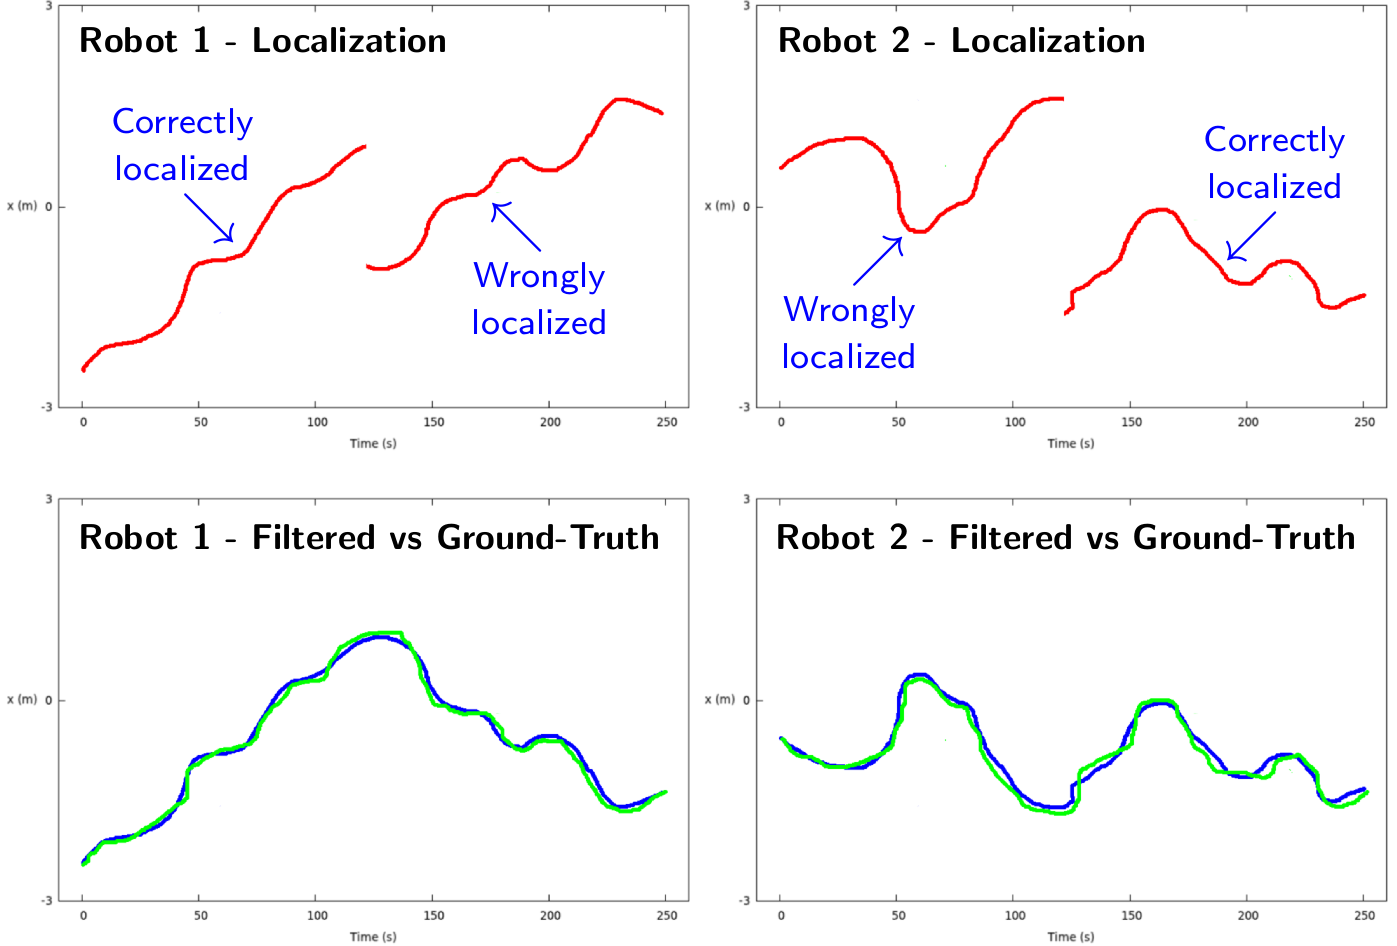
\includegraphics[scale=0.15]{Figures/LocalisationResults}
			};
		\end{tikzpicture}
	\end{center}
	
	\vspace{0.512cm}
	
	\tiny
	
	\textbf{Disambiguating Localization Symmetry through a Multi-Clustered Particle Filtering} \\
	F. Previtali, G. Gemignani, L. Iocchi, D. Nardi \\
	\emph{IEEE International Conference on Multisensor Fusion and Integration for Intelligent Systems,
	2015} \\
\end{frame}

%\begin{frame}
%	\frametitle{Challenge}
%	
%	\Large
%	
%	\vspace{0.25cm}
%	
%	\begin{figure}
%		\centering
%		\begin{tikzpicture}
%			\node at (0,0) [draw=white,ultra thick,inner sep=0pt]
%			{
%				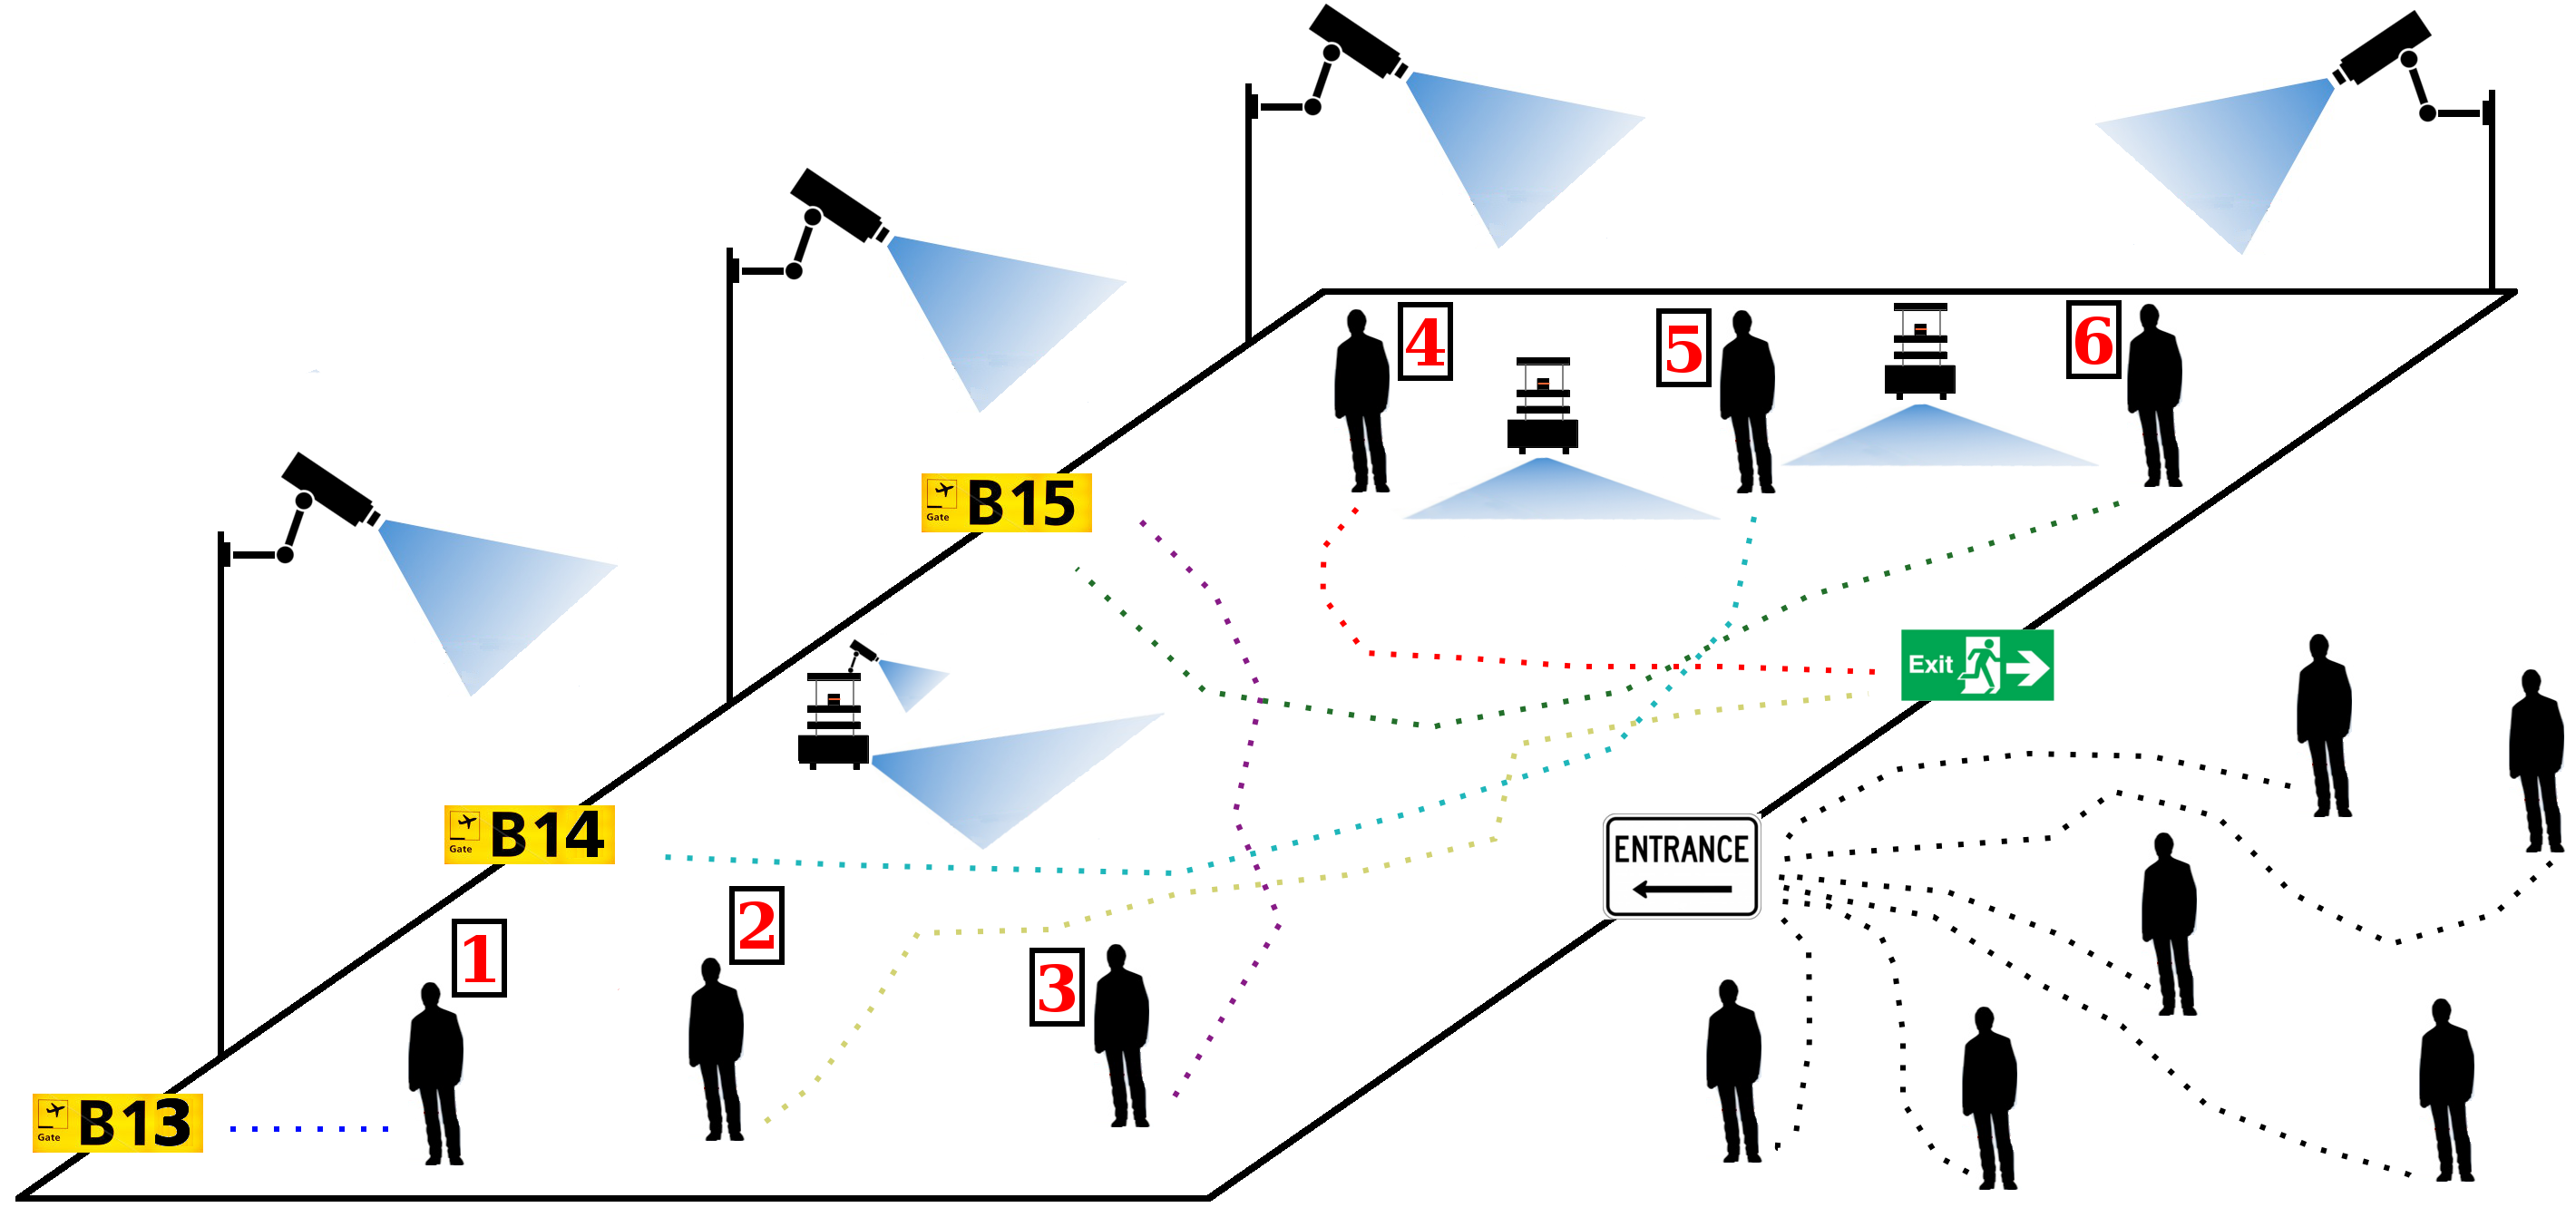
\includegraphics[width=0.8\linewidth]{Figures/Challenge}
%			};
%		\end{tikzpicture}
%	\end{figure}
%	
%	\vspace{-0.4cm}
%	
%	\begin{center}
%		What is the real position of the blue robot number 3?
%	\end{center}
%\end{frame}
%
%\begin{frame}
%	\frametitle{Quantitative Evaluation}
%	\framesubtitle{RoboCup Domain}
%	
%	\large
%	
%	\vspace{-0.85cm}
%	
%	Simulating 3 Aldebaran Nao robots playing soccer, one of them alternatively forced to be inversely
%	localised
%	
%	\Large
%	
%	\vspace{-0.6cm}
%	
%	\begin{columns}[T]
%		\column{1.02\textwidth}
%		
%	\begin{figure}
%		\centering
%		
%		\begin{tikzpicture}
%			\node at (0,0) [draw=white,ultra thick,inner sep=0pt]
%			{
%				\includegraphics[width=0.34\linewidth]{Figures/Result-Scenario-2_Robot-1}
%			};
%			\node at (4.1,0) [draw=white,ultra thick,inner sep=0pt]
%			{
%				\includegraphics[width=0.34\linewidth]{Figures/Result-Scenario-2_Robot-2}
%			};
%			\node at (0,-2.9) [draw=white,ultra thick,inner sep=0pt]
%			{
%				\includegraphics[width=0.34\linewidth]{Figures/Result-Scenario-2_Robot-1-GT}
%			};
%			\node at (4.1,-2.9) [draw=white,ultra thick,inner sep=0pt]
%			{
%				\includegraphics[width=0.34\linewidth]{Figures/Result-Scenario-2_Robot-2-GT}
%			};
%			\node at (8.2,0) [draw=white,ultra thick,inner sep=0pt]
%			{
%				\includegraphics[width=0.34\linewidth]{Figures/Result-Scenario-2_Robot-3}
%			};
%			\node at (8.2,-2.9) [draw=white,ultra thick,inner sep=0pt]
%			{
%				\includegraphics[width=0.34\linewidth]{Figures/Result-Scenario-2_Robot-3-GT}
%			};
%		\end{tikzpicture}
%	\end{figure}
%	\end{columns}
%	
%	\vspace{-6.15cm}
%	
%	\begin{tabbing}
%		\hspace{0.21cm}
%		\tiny
%		\textbf{Robot 1 - Localization}
%		\hspace{1.79cm}
%		\textbf{Robot 2 - Localization}
%		\hspace{1.79cm}
%		\textbf{Robot 3 - Localization}
%	\end{tabbing}
%	
%	\vspace{-1cm}
%	
%	\begin{tabbing}
%		\hspace{0.4cm}
%		\tiny
%		\textcolor{blue}{Correctly}
%	\end{tabbing}
%	
%	\vspace{-1.2cm}
%	
%	\begin{tabbing}
%		\hspace{0.42cm}
%		\tiny
%		\textcolor{blue}{localized}
%	\end{tabbing}
%	
%	\vspace{-1.17cm}
%	
%	\begin{tabbing}
%		\footnotesize
%		\hspace{0.87cm}
%		\textcolor{blue}{$ \searrow $}
%	\end{tabbing}
%	
%	\vspace{-1.43cm}
%	
%	\begin{tabbing}
%		\footnotesize
%		\hspace{2.68cm}
%		\textcolor{blue}{$ \nwarrow $}
%	\end{tabbing}
%	
%	\vspace{-1.2cm}
%	
%	\begin{tabbing}
%		\hspace{2.53cm}
%		\tiny
%		\textcolor{blue}{Wrongly}
%	\end{tabbing}
%	
%	\vspace{-1.2cm}
%	
%	\begin{tabbing}
%		\hspace{2.52cm}
%		\tiny
%		\textcolor{blue}{localized}
%	\end{tabbing}
%	
%	\vspace{-1.83cm}
%	
%	\begin{tabbing}
%		\footnotesize
%		\hspace{4.8cm}
%		\textcolor{blue}{$ \nearrow $}
%	\end{tabbing}
%	
%	\vspace{-1.2cm}
%	
%	\begin{tabbing}
%		\hspace{4.35cm}
%		\tiny
%		\textcolor{blue}{Wrongly}
%	\end{tabbing}
%	
%	\vspace{-1.2cm}
%	
%	\begin{tabbing}
%		\hspace{4.34cm}
%		\tiny
%		\textcolor{blue}{localized}
%	\end{tabbing}
%	
%	\vspace{-2.75cm}
%	
%	\begin{tabbing}
%		\hspace{6.82cm}
%		\tiny
%		\textcolor{blue}{Correctly}
%	\end{tabbing}
%	
%	\vspace{-1.2cm}
%	
%	\begin{tabbing}
%		\hspace{6.84cm}
%		\tiny
%		\textcolor{blue}{localized}
%	\end{tabbing}
%	
%	\vspace{-1.17cm}
%	
%	\begin{tabbing}
%		\footnotesize
%		\hspace{7cm}
%		\textcolor{blue}{$ \swarrow $}
%	\end{tabbing}
%	
%	\vspace{-1.79cm}
%	
%	\begin{tabbing}
%		\hspace{9.52cm}
%		\tiny
%		\textcolor{blue}{Correctly}
%	\end{tabbing}
%	
%	\vspace{-1.2cm}
%	
%	\begin{tabbing}
%		\hspace{9.54cm}
%		\tiny
%		\textcolor{blue}{localized}
%	\end{tabbing}
%	
%	\vspace{-1.17cm}
%	
%	\begin{tabbing}
%		\footnotesize
%		\hspace{9.99cm}
%		\textcolor{blue}{$ \searrow $}
%	\end{tabbing}
%	
%	\vspace{0.01cm}
%	
%	\begin{tabbing}
%		\hspace{0.21cm}
%		\tiny
%		\textbf{Robot 1 - Filtered vs Ground-Truth}
%		\hspace{0.53cm}
%		\textbf{Robot 2 - Filtered vs Ground-Truth}
%		\hspace{0.53cm}
%		\textbf{Robot 3 - Filtered vs Ground-Truth}
%	\end{tabbing}
%\end{frame}
%
%\begin{frame}
%	\frametitle{Qualitative Evaluation}
%	\framesubtitle{RoboCup Iran Open}
%	
%	\begin{figure}[!h]
%		\centering
%		\includemovie[inline=false,text=
%		{
%			\begin{tikzpicture}
%				\node at (0,0) [draw=black,ultra thick,inner sep=0pt]
%				{
%					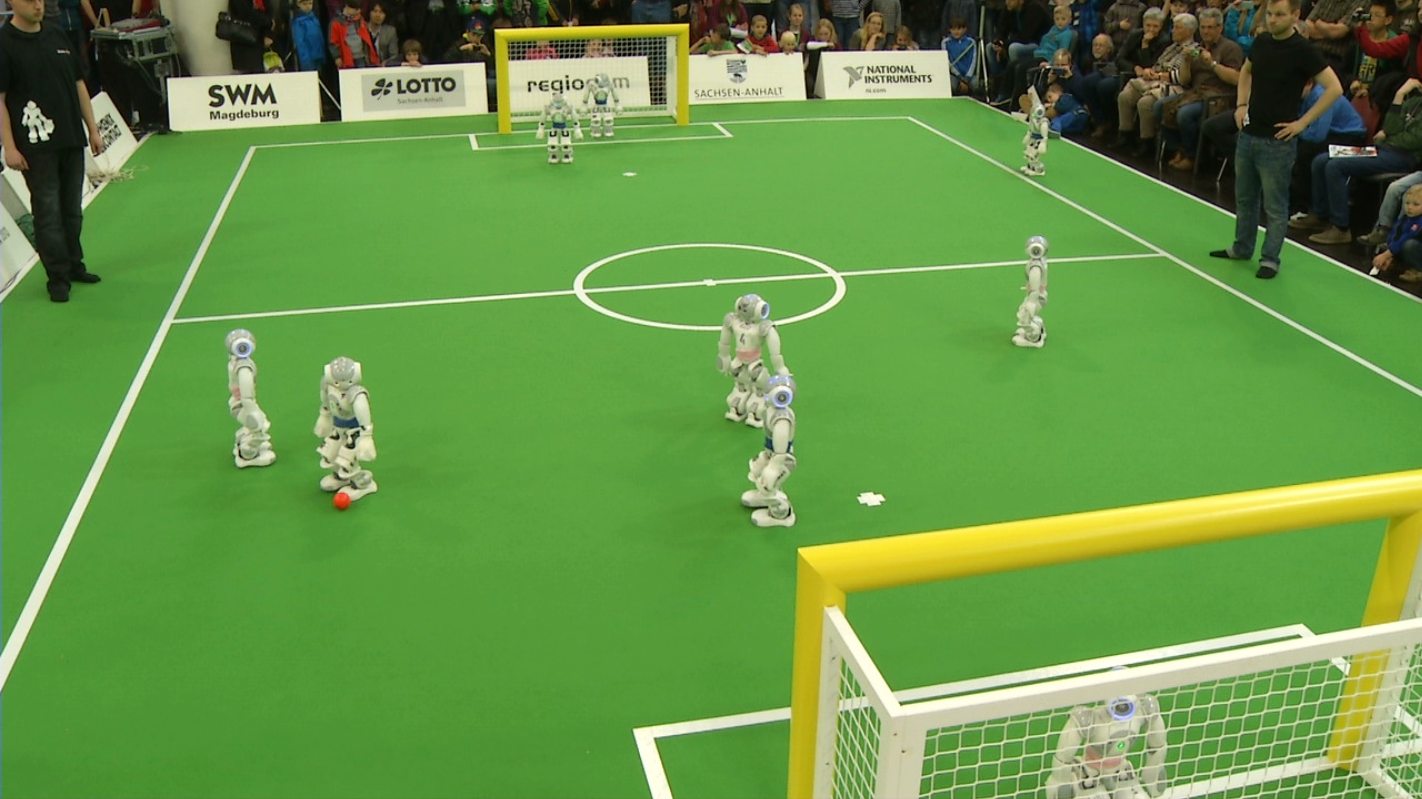
\includegraphics[width=0.85\linewidth]{Figures/Nao}
%				};
%			\end{tikzpicture}
%		}]{}{}{../Videos/2-Nao/PTracking-RLSD.avi}
%	\end{figure}
%\end{frame}

\begin{frame}
	\frametitle{Experimental Evaluation}
	\framesubtitle{Multi-Sensor, Multi-Object}
	
	\vspace{0.2cm}
	
	\begin{center}
		\begin{tikzpicture}
			\node at (-2.5,0) [draw=black,ultra thick,inner sep=0pt]
			{
				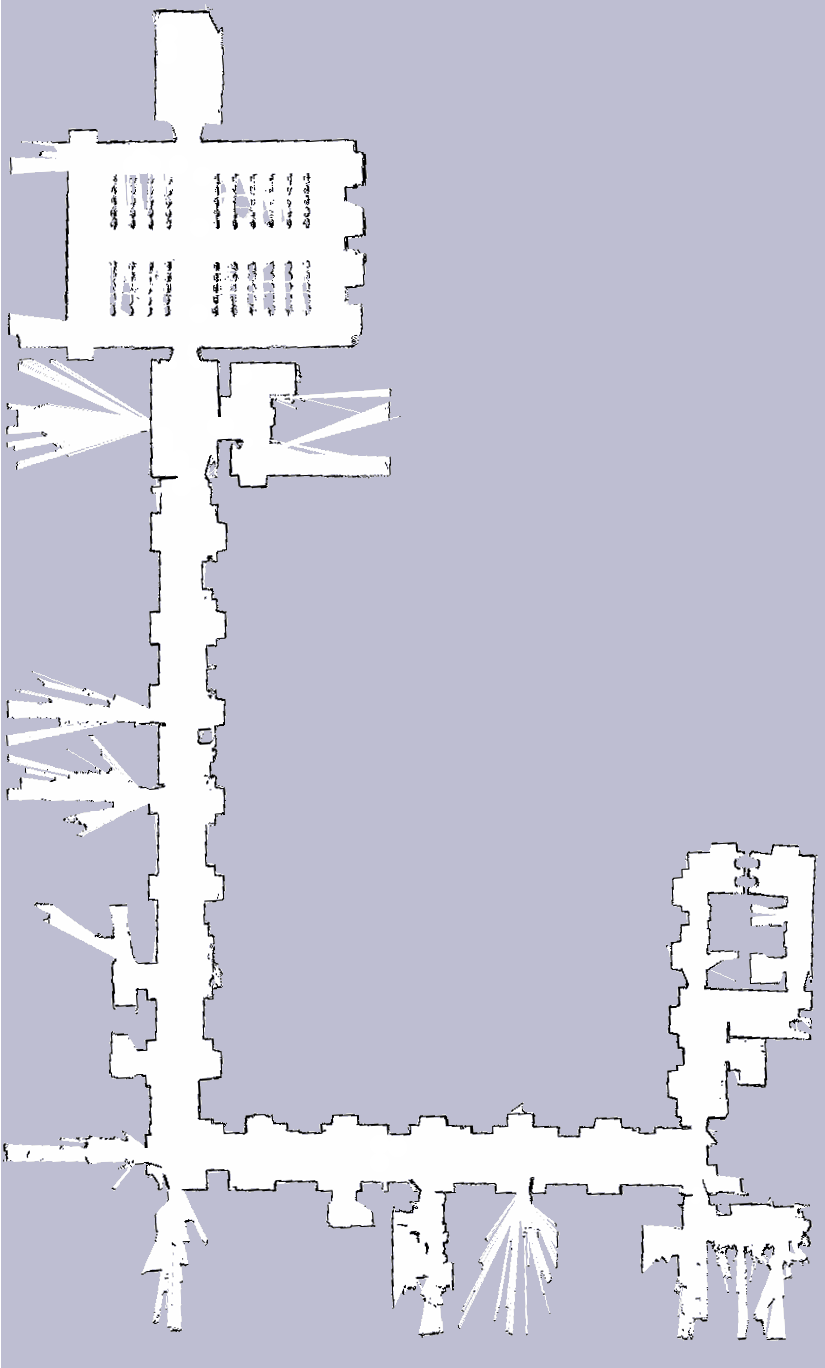
\includegraphics[height=2.7cm]{Figures/Map-1}
			};
			\node at (2.5,0) [draw=black,ultra thick,inner sep=0pt]
			{
				\includegraphics[height=2.7cm]{Figures/Map-2}
			};
		\end{tikzpicture}
	\end{center}
	
	\tiny
	
	\vspace{-0.15cm}
	
	\begin{table}[!t]
		\centering
		\def\arraystretch{1.15}
		\setlength{\tabcolsep}{0.15cm}
		\begin{tabular}{ccccc|ccccc}
			\cline{1-9}
			\multicolumn{9}{c}{\textbf{\begin{tabular}[c]
			{@{}c@{}}Tracking Performance (MOTA,MOTP)\end{tabular}}} \\ \cline{1-9}
			\multicolumn{1}{l}{} & \multicolumn{4}{c|}{\textbf{\begin{tabular}[c]
			{@{}c@{}}DIAG\end{tabular}}} &
			\multicolumn{4}{c}{\textbf{\begin{tabular}[c]
			{@{}c@{}}Peccioli\end{tabular}}} \\ \hline
			\multicolumn{1}{c|}{\textbf{\#}} & \textbf{Setting 1} & \textbf{Setting 2} &
			\textbf{Setting 3} & \textbf{Setting 4} & \textbf{Setting 1} & \textbf{Setting 2} &
			\textbf{Setting 3} & \textbf{Setting 4} \\
			
			\multicolumn{1}{c|}{1} & (0.63,0.45) & (0.67,0.49) & (0.75,0.51) & (0.94,0.75)
								   & (0.67,0.42) & (0.71,0.49) & (0.78,0.58) & (0.93,0.79) \\
			\multicolumn{1}{c|}{2} & (0.59,0.42) & (0.65,0.45) & (0.73,0.49) & (0.92,0.74)
								   & (0.64,0.47) & (0.73,0.51) & (0.72,0.52) & (0.96,0.79) \\
			\multicolumn{1}{c|}{3} & (0.64,0.41) & (0.69,0.48) & (0.70,0.47) & (0.95,0.77)
								   & (0.64,0.47) & (0.73,0.51) & (0.72,0.52) & (0.96,0.79) \\
			\multicolumn{1}{c|}{4} & (0.62,0.45) & (0.62,0.40) & (0.74,0.50) & (0.92,0.75)
								   & (0.66,0.44) & (0.68,0.43) & (0.75,0.53) & (0.93,0.77) \\
			\multicolumn{1}{c|}{5} & (0.57,0.39) & (0.64,0.44) & (0.70,0.48) & (0.94,0.77)
								   & (0.60,0.41) & (0.65,0.45) & (0.71,0.51) & (0.97,0.81) \\
			\hline
		\end{tabular}
	\end{table}
	
	\vspace{0.455cm}
	
	\tiny
	
	\textbf{PTracking: Distributed Multi-Agent Multi-Object Tracking through Multi-Clustered Particle
	Filtering} \\
	F. Previtali, L. Iocchi \\
	\emph{IEEE International Conference on Multisensor Fusion and Integration for Intelligent Systems,
	2015} \\
\end{frame}

\begin{frame}
	\frametitle{Experimental Evaluation}
	\framesubtitle{Multi-Sensor, Multi-Object}
	
	\vspace{0.1cm}
	
	\begin{center}
		\begin{tikzpicture}
			\node at (0,0) [draw=black,ultra thick,inner sep=0pt]
			{
				\includegraphics[height=2.9cm]{Figures/Boat-1}
			};
			\node at (3.7,0) [draw=black,ultra thick,inner sep=0pt]
			{
				\includegraphics[height=2.9cm]{Figures/Boat-2}
			};
			\node at (7.45,0) [draw=black,ultra thick,inner sep=0pt]
			{
				\includegraphics[height=2.9cm]{Figures/Boat-3}
			};
		\end{tikzpicture}
	\end{center}
	
	\vspace{-0.2cm}
	
	\footnotesize
	
	\begin{table}
		\centering
		\def\arraystretch{1.15}
		\setlength{\tabcolsep}{0.15cm}
		\begin{tabular}{cccc}
			\cline{1-4}
			\multicolumn{4}{c}{\textbf{PTracking}} \\ \cline{1-4}
			\textbf{Video} & \textbf{Multi-Source} & \textbf{MOTA} & \textbf{MOTP} \\
			\hline
			occlusions-1 (left) & NO & 0.815 & 0.613 \\
			\hline
			occlusions-1 (left) & YES & 0.975 & 0.871 \\
			\hline
			occlusions-2 (center) & NO & 0.910 & 0.554 \\
			\hline
			high-view (right) & NO & 0.910 & 0.604 \\
			\hline
		\end{tabular}
	\end{table}
	
	\vspace{-0.04cm}
	
	\tiny
	
	\textbf{Enhancing Automatic Maritime Surveillance Systems with Visual Information} \\
	D. D. Bloisi, F. Previtali, A. Pennisi, D. Nardi, M. Fiorini \\
	\emph{IEEE Transaction on Intelligent Transportation Systems} [second revision] \\
\end{frame}

\begin{frame}
	\frametitle{Qualitative Evaluation}
	\framesubtitle{Maritime Domain - Multiple Source Data Fusion}
	
	\begin{figure}[!h]
		\centering
		\includemovie[inline=false,text=
		{
			\begin{tikzpicture}
				\node at (0,0) [draw=black,ultra thick,inner sep=0pt]
				{
					\includegraphics[width=0.65\linewidth]{Figures/Boat-1}
				};
			\end{tikzpicture}
		}]{}{}{../Videos/1-Boat/PTracking-DataFusion.avi}
	\end{figure}
\end{frame}

\begin{frame}
	\frametitle{Experimental Evaluation}
	\framesubtitle{Multi-Sensor, Multi-Object}
	
	\vspace{0.2cm}
	
	\begin{center}
		\begin{tikzpicture}
			\node at (-2.04,0) [draw=black,ultra thick,inner sep=0pt]
			{
				\includegraphics[height=2.5cm]{Figures/PETS2009-7}
			};
			\node at (2.04,0) [draw=black,ultra thick,inner sep=0pt]
			{
				\includegraphics[height=2.5cm]{Figures/IssiaSoccer-Camera1}
			};
		\end{tikzpicture}
	\end{center}
	
	\tiny
	
	\vspace{-0.3cm}

	\begin{table}[!t]
		\renewcommand{\arraystretch}{1.25}
		\setlength{\tabcolsep}{0.14cm}
		\centering
		\begin{tabular}{ccccc|cccc}
			\cline{1-9}
			\multicolumn{5}{c|}{\textbf{PETS 2009}} & \multicolumn{4}{c}{\textbf{Issia Soccer}} \\
			\hline
			\textbf{Method} & \textbf{MOTA} & \textbf{MOTP} & \textbf{Type} & \textbf{Real-Time} &
			\textbf{Method} & \textbf{Camera} & \textbf{MOTA} & \textbf{MOTP} \\
			Leal-Taix\'{e} \cite{Leal11} & 0.67 & 0.534 & OFFLINE & NO & PTracking & 1 & 0.723 & 0.612
			\\
			Berclaz \cite{Berclaz11} & 0.732 & 0.603 & OFFLINE & NO & PTracking & 1, 2 & 0.789 & 0.638
			\\
			Henriques \cite{Henriques11} & 0.833 & 0.711 & OFFLINE & NO & PTracking & 1, 2, 3 & 0.817 &
			0.651 \\
			Breitenstein \cite{Breitenstein11} & 0.745 & 0.563 & ONLINE & NO & PTracking & 1, 2, 3, 4 &
			0.894 & 0.706 \\
			Yang \cite{Yang09} & 0.759 & 0.538 & ONLINE & NO \\
			Bae \cite{Bae14} & 0.830 & 0.696 & ONLINE & \textbf{YES} \\
			PTracking & \textbf{0.874} & \textbf{0.722} & ONLINE & \textbf{YES (30.2 FPS)} \\
			PTracking$^*$ & \textbf{0.882} & \textbf{0.717} & ONLINE & NO (11.8 FPS) \\
			\hline
		\end{tabular}
	\end{table}
	
	\tiny
	
	\textbf{A Distributed Approach for Real-Time Multi-Camera Multi-Object Tracking} \\
	F. Previtali, D. D. Bloisi, L. Iocchi \\
	\emph{Journal on Machine Vision and Applications} [submitted] \\
\end{frame}

\begin{frame}
	\frametitle{Experimental Evaluation}
	\framesubtitle{Multi-Sensor, Multi-Object}
	
	\begin{center}
		\begin{tikzpicture}
			\node at (-2.54,0) [draw=black,ultra thick,inner sep=0pt]
			{
				\includegraphics[height=2.3cm]{Figures/RFID}
			};
			\node at (2.54,0) [draw=black,ultra thick,inner sep=0pt]
			{
				\includegraphics[height=2.3cm]{Figures/Environment}
			};
		\end{tikzpicture}
	\end{center}
	
	\scriptsize
	
	\vspace{-0.254cm}
	
	\begin{table}[!t]
		\centering
		\renewcommand{\arraystretch}{1.1}
		\setlength{\tabcolsep}{0.09cm}
		\begin{tabular}{c c c | c c c}
			\cline{1-6}
			\multicolumn{6}{c}{\textbf{PTracking}} \\ \hline
			\textbf{Experiment} & \textbf{MOTA} & \textbf{MOTP} & \textbf{Experiment} & \textbf{MOTA} & \textbf{MOTP} \\
			\hline
			1 & 0.95 & 0.85 & 6 & 0.91 & 0.87 \\
			2 & 0.97 & 0.90 & 7 & 0.95 & 0.89 \\
			3 & 0.96 & 0.88 & 8 & 0.95 & 0.91 \\
			4 & 0.92 & 0.91 & 9 & 0.97 & 0.93 \\
			5 & 0.99 & 0.95 & 10 & 0.98 & 0.92 \\
			\hline
		\end{tabular}
	\end{table}
	
	\tiny
	
	\textbf{Multi-Robot Surveillance through a Distributed Sensor Network} \\
	A. Pennisi, F. Previtali, F. Ficarola, D. D. Bloisi, L. Iocchi, A. Vitaletti \\
	\emph{Studies in Computational Intelligence, 2015} \\
	
	\vspace{0.1cm}
	
	\textbf{Distributed Sensor Network for Multi-Robot Surveillance} \\
	A. Pennisi, F. Previtali, F. Ficarola, D. D. Bloisi, L. Iocchi, A. Vitaletti \\
	\emph{Procedia Computer Science, 2014} \\
\end{frame}

%\begin{frame}
%	\frametitle{Qualitative Evaluation}
%	\framesubtitle{Maritime Domain - Blue Water}
%	
%	\begin{figure}[!h]
%		\centering
%		\includemovie[inline=false,text=
%		{
%			\begin{tikzpicture}
%				\node at (0,0) [draw=black,ultra thick,inner sep=0pt]
%				{
%					\includegraphics[width=0.65\linewidth]{Figures/Boat-2}
%				};
%			\end{tikzpicture}
%		}]{}{}{../Videos/1-Boat/PTracking-Wester_LLTV_VELA.avi}
%	\end{figure}
%\end{frame}
%
%\begin{frame}
%	\frametitle{Experimental Evaluation}
%	\framesubtitle{Multi-Sensor, Multi-Object}
%	
%	\large
%	
%	\vspace{-0.35cm}
%	
%	\begin{columns}[t]
%		\only<1->
%		{
%			\column{0.8\textwidth}
%			
%			\begin{block}{Issia Soccer}
%				tracking of players in a real soccer match
%			\end{block}
%			
%			\column{0.15\textwidth}
%		}
%	\end{columns}
%	
%	\begin{center}
%		\begin{tikzpicture}
%			\node at (2.39,0) [draw=black,ultra thick,inner sep=0pt]  {\includegraphics[height=2.1cm]{Figures/IssiaSoccer-Camera1}};
%			\node at (6.26,0) [draw=black,ultra thick,inner sep=0pt]  {\includegraphics[height=2.1cm]{Figures/IssiaSoccer-Camera2}};
%			\node at (2.39,-2.22) [draw=black,ultra thick,inner sep=0pt]  {\includegraphics[height=2.1cm]{Figures/IssiaSoccer-Camera3}};
%			\node at (6.26,-2.22) [draw=black,ultra thick,inner sep=0pt]  {\includegraphics[height=2.1cm]{Figures/IssiaSoccer-Camera4}};
%		\end{tikzpicture}
%	\end{center}
%	
%	\vspace{-0.05cm}
%	
%	\tiny
%	
%	\textbf{A Distributed Approach for Real-Time Multi-Camera Multi-Object Tracking} \\
%	F. Previtali, D. D. Bloisi, L. Iocchi \\
%	\emph{Journal on Computer Vision and Image Understanding} [second revision] \\
%\end{frame}
%
%\begin{frame}
%	\frametitle{Quantitative Evaluation}
%	\framesubtitle{People Domain - Issia Soccer}
%	
%	\Large
%	
%	\begin{table}[!t]
%		\renewcommand{\arraystretch}{1.3}
%		\centering
%		\begin{tabular}{lcccc}
%			\hline
%			\hline
%			\multicolumn{1}{c}{\begin{tabular}[c]{@{}c@{}}\textbf{Method} \end{tabular}} & \textbf{MOTA} & \textbf{MOTP} \\
%			\hline
%			PTracking - Camera 1 & 0.723 & 0.612 \\
%			\hline
%			PTracking - Camera 1, 2 & 0.789 & 0.638 \\
%			\hline
%			PTracking - Camera 1, 2, 3 & 0.817 & 0.651 \\
%			\hline
%			PTracking - Camera 1, 2, 3, 4 & 0.894 & 0.706 \\
%			\hline
%		\hline
%		\end{tabular}
%	\end{table}
%\end{frame}
%
%\begin{frame}
%	\frametitle{Qualitative Evaluation}
%	\framesubtitle{People Domain - Issia Soccer}
%	
%	\begin{figure}[!h]
%		\centering
%		\includemovie[inline=false,text=
%		{
%			\begin{tikzpicture}
%				\node at (0,0) [draw=black,ultra thick,inner sep=0pt]
%				{
%					\includegraphics[width=0.85\linewidth]{Figures/IssiaSoccer-Camera1}
%				};
%			\end{tikzpicture}
%		}]{}{}{../Videos/4-People/PTracking-IssiaSoccer.mp4}
%	\end{figure}
%\end{frame}
%
%\begin{frame}
%	\frametitle{Experimental Evaluation}
%	\framesubtitle{Multi-Sensor, Multi-Object}
%	
%	\large
%	
%	\vspace{-0.45cm}
%	
%	\begin{columns}[t]
%		\only<1->
%		{
%			\column{0.8\textwidth}
%			
%			\begin{block}{PETS-2009}
%				tracking of individuals within a crowd
%			\end{block}
%			
%			\column{0.15\textwidth}
%		}
%	\end{columns}
%	
%	\vspace{0.1cm}
%	
%	\begin{center}
%		\begin{tikzpicture}
%			\node at (0,0) [draw=black,ultra thick,inner sep=0pt]  {\includegraphics[height=2.55cm]{Figures/PETS2009-1}};
%			\node at (3.55,0) [draw=black,ultra thick,inner sep=0pt]  {\includegraphics[height=2.55cm]{Figures/PETS2009-3}};
%			\node at (7.17,0) [draw=black,ultra thick,inner sep=0pt]  {\includegraphics[height=2.55cm]{Figures/PETS2009-6}};
%			\node at (1.8,-2.7) [draw=black,ultra thick,inner sep=0pt]  {\includegraphics[height=2.55cm]{Figures/PETS2009-7}};
%			\node at (5.5,-2.7) [draw=black,ultra thick,inner sep=0pt]  {\includegraphics[height=2.55cm]{Figures/PETS2009-8}};
%		\end{tikzpicture}
%	\end{center}
%\end{frame}
%
%\begin{frame}
%	\frametitle{Quantitative Evaluation}
%	\framesubtitle{People Domain - PETS-2009}
%	
%	\large
%	
%	\begin{table}[!t]
%		\renewcommand{\arraystretch}{1.3}
%		\centering
%		\begin{tabular}{ccccc}
%			\hline
%			\hline
%			\textbf{Method} & \textbf{MOTA} & \textbf{MOTP} & \textbf{Type} & \textbf{Real-Time} \\
%			\hline
%			Leal-Taix\'{e} \cite{Leal11} & 0.67 & 0.534 & OFFLINE & NO \\
%			\hline
%			Berclaz \cite{Berclaz11} & 0.732 & 0.603 & OFFLINE & NO \\
%			\hline
%			Henriques \cite{Henriques11} & 0.833 & 0.711 & OFFLINE & NO \\
%			\hline
%			Breitenstein \cite{Breitenstein11} & 0.745 & 0.563 & ONLINE & NO \\
%			\hline
%			Yang \cite{Yang09} & 0.759 & 0.538 & ONLINE & NO \\
%			\hline
%			Bae \cite{Bae14} & 0.830 & 0.696 & ONLINE & \textbf{YES} \\
%			\hline
%			PTracking & \textbf{0.874} & \textbf{0.722} & ONLINE & \textbf{YES (30.2 FPS)} \\
%			\hline
%			PTracking$^*$ & \textbf{0.882} & \textbf{0.717} & ONLINE & NO (11.8 FPS) \\
%			\hline
%		\hline
%		\end{tabular}
%	\end{table}
%\end{frame}
%
%\begin{frame}
%	\frametitle{Experimental Evaluation}
%	\framesubtitle{Multi-Sensor, Multi-Object}
%	
%	\large
%	
%	\begin{columns}[t]
%		\only<1->
%		{
%			\column{0.8\textwidth}
%			
%			\begin{block}{Prey-Predator Game}
%				demonstrating the advantages of using mobile sensors
%			\end{block}
%			
%			\column{0.15\textwidth}
%		}
%	\end{columns}
%	
%	\vspace{0.1cm}
%	
%	\begin{center}
%		\begin{tikzpicture}
%			\node at (0,0) [draw=black,ultra thick,inner sep=0pt]  {\includegraphics[height=3.25cm]{Figures/Map-1}};
%			\node at (6,0) [draw=black,ultra thick,inner sep=0pt]  {\includegraphics[height=3.25cm]{Figures/Map-2}};
%		\end{tikzpicture}
%	\end{center}
%	
%	\vspace{0.52cm}
%	
%	\tiny
%	
%	\textbf{PTracking: Distributed Multi-Agent Multi-Object Tracking through Multi-Clustered Particle
%	Filtering} \\
%	F. Previtali, L. Iocchi \\
%	\emph{IEEE International Conference on Multisensor Fusion and Integration for Intelligent Systems,
%	2015} \\
%\end{frame}
%
%\begin{frame}
%	\frametitle{Quantitative Evaluation}
%	\framesubtitle{DIAG}
%	
%	\small
%	
%	\begin{table}[!t]
%		\centering
%		\begin{tabular}{ccccc}
%			\cline{1-5}
%			\multicolumn{1}{l}{} & \multicolumn{4}{c}{\textbf{\begin{tabular}[c]{@{}c@{}}
%			Prey-Predator Distance (avg $ \pm $ std. dev.)\end{tabular}}} \\ \hline
%			\multicolumn{1}{c}{\textbf{\#}} & \textbf{Setting 1} & \textbf{Setting 2} &
%			\textbf{Setting 3} & \textbf{Setting 4} \\
%			
%			\multicolumn{1}{c}{1} & 3.04 $ \pm $ 0.63 $ m $ & 2.70 $ \pm $ 0.49
%								  $ m $ & 2.02 $ \pm $ 0.38 $ m $ & 1.12 $ \pm $
%								  0.19 $ m $ \\
%			\multicolumn{1}{c}{2} & 2.95 $ \pm $ 0.80 $ m $ & 2.65 $ \pm $ 0.48
%								  $ m $ & 1.95 $ \pm $ 0.42 $ m $ & 1.15 $ \pm $
%								  0.20 $ m $ \\
%			\multicolumn{1}{c}{3} & 3.12 $ \pm $ 0.53 $ m $ & 2.87 $ \pm $ 0.56
%								  $ m $ & 2.03 $ \pm $ 0.41 $ m $ & 1.13 $ \pm $
%								  0.19 $ m $ \\
%			\multicolumn{1}{c}{4} & 3.01 $ \pm $ 0.69 $ m $ & 2.73 $ \pm $ 0.49
%								  $ m $ & 2.06 $ \pm $ 0.38 $ m $ & 1.08 $ \pm $
%								  0.22 $ m $ \\
%			\multicolumn{1}{c}{5} & 2.99 $ \pm $ 0.72 $ m $ & 2.86 $ \pm $ 0.61
%								  $ m $ & 1.99 $ \pm $ 0.40 $ m $ & 1.11 $ \pm $
%								  0.17 $ m $ \\
%			\hline
%			
%			\\
%			
%			\hline
%			\multicolumn{1}{l}{} & \multicolumn{4}{c}{\textbf{\begin{tabular}[c]
%			{@{}c@{}}Tracking Performance (MOTA,MOTP)\end{tabular}}} \\ \hline
%			\multicolumn{1}{c}{\textbf{\#}} & \textbf{Setting 1} & \textbf{Setting 2} &
%			\textbf{Setting 3} & \textbf{Setting 4} \\
%			
%			\multicolumn{1}{c}{1} & (0.63,0.45) & (0.67,0.49) & (0.75,0.51) & (0.94,0.75) \\
%			\multicolumn{1}{c}{2} & (0.59,0.42) & (0.65,0.45) & (0.73,0.49) & (0.92,0.74) \\
%			\multicolumn{1}{c}{3} & (0.64,0.41) & (0.69,0.48) & (0.70,0.47) & (0.95,0.77) \\
%			\multicolumn{1}{c}{4} & (0.62,0.45) & (0.62,0.40) & (0.74,0.50) & (0.92,0.75) \\
%			\multicolumn{1}{c}{5} & (0.57,0.39) & (0.64,0.44) & (0.70,0.48) & (0.94,0.77) \\
%			\hline
%		\end{tabular}
%	\end{table}
%\end{frame}
%
%\begin{frame}
%	\frametitle{Quantitative Evaluation}
%	\framesubtitle{Peccioli House}
%	
%	\small
%	
%	\begin{table}
%		\centering
%		\begin{tabular}{ccccc}
%			\cline{1-5}
%			\multicolumn{1}{l}{} & \multicolumn{4}{c}{\textbf{\begin{tabular}[c]{@{}c@{}}
%			Prey-Predator Distance (avg $ \pm $ std. dev.)\end{tabular}}} \\ \hline
%			\multicolumn{1}{c}{\textbf{\#}} & \textbf{Setting 1} & \textbf{Setting 2} &
%			\textbf{Setting 3} & \textbf{Setting 4} \\
%			
%			\multicolumn{1}{c}{1} & 2.84 $ \pm $ 0.59 $ m $ & 2.55 $ \pm $ 0.47
%								  $ m $ & 1.85 $ \pm $ 0.38 $ m $ & 1.07 $ \pm $
%								  0.18 $ m $ \\
%			\multicolumn{1}{c}{2} & 2.85 $ \pm $ 0.74 $ m $ & 2.52 $ \pm $ 0.51
%								  $ m $ & 1.84 $ \pm $ 0.40 $ m $ & 1.05 $ \pm $
%								  0.21 $ m $ \\
%			\multicolumn{1}{c}{3} & 3.03 $ \pm $ 0.57 $ m $ & 2.76 $ \pm $ 0.52
%								  $ m $ & 1.91 $ \pm $ 0.43 $ m $ & 1.11 $ \pm $
%								  0.20 $ m $ \\
%			\multicolumn{1}{c}{4} & 3.04 $ \pm $ 0.61 $ m $ & 2.63 $ \pm $ 0.47
%								  $ m $ & 1.93 $ \pm $ 0.39 $ m $ & 1.08 $ \pm $
%								  0.21 $ m $ \\
%			\multicolumn{1}{c}{5} & 2.89 $ \pm $ 0.68 $ m $ & 2.77 $ \pm $ 0.56
%								  $ m $ & 1.89 $ \pm $ 0.41 $ m $ & 1.09 $ \pm $
%								  0.15 $ m $ \\
%			
%			\hline
%			
%			\\
%			
%			\hline
%			\multicolumn{1}{l}{} & \multicolumn{4}{c}{\textbf{\begin{tabular}[c]
%			{@{}c@{}}Tracking Performance (MOTA,MOTP)\end{tabular}}} \\ \hline
%			\multicolumn{1}{c}{\textbf{\#}} & \textbf{Setting 1} & \textbf{Setting 2} &
%			\textbf{Setting 3} & \textbf{Setting 4} \\
%			
%			\multicolumn{1}{c}{1} & (0.67,0.42) & (0.71,0.49) & (0.78,0.58) & (0.93,0.79) \\
%			\multicolumn{1}{c}{2} & (0.62,0.43) & (0.69,0.46) & (0.77,0.55) & (0.95,0.76) \\
%			\multicolumn{1}{c}{3} & (0.64,0.47) & (0.73,0.51) & (0.72,0.52) & (0.96,0.79) \\
%			\multicolumn{1}{c}{4} & (0.66,0.44) & (0.68,0.43) & (0.75,0.53) & (0.93,0.77) \\
%			\multicolumn{1}{c}{5} & (0.60,0.41) & (0.65,0.45) & (0.71,0.51) & (0.97,0.81) \\
%			\hline
%		\end{tabular}
%	\end{table}
%\end{frame}

\section{Related Work - Activity Forecasting}

\begin{frame}
	\frametitle{Related Work}
	\framesubtitle{Human Activity Classification and Activity Recognition}
	
	\vspace{0.4cm}
	
	\begin{columns}[T]
		\column{.55\textwidth}
		
		\vspace{0.2cm}
		
		\begin{itemize}
			\item \textbf{Nascimento {et al.} \cite{Nascimento10}:} recognise pedestrian trajectories in
				  video sequences, in a surveillance context
			
			\vspace{1.2cm}
			
			\item \textbf{Veloso {et al.} \cite{Vail07}:} discriminatively trained Conditional Random
				  Fields for activity recognition
		\end{itemize}
		
		\column{.5\textwidth}
		
		\centering
		\begin{tikzpicture}
			\node at (1.42,0) [draw=black,ultra thick,inner sep=0pt]
			{
				\includegraphics[height=2.2cm]{Figures/Nascimento-1}
			};
			\node at (-1.42,0) [draw=black,ultra thick,inner sep=0pt]
			{
				\includegraphics[height=2.2cm]{Figures/Nascimento-2}
			};
			\node at (0,-2.8) [draw=black,ultra thick,inner sep=0pt]
			{
				\includegraphics[width=3.6cm]{Figures/Veloso}
			};
		\end{tikzpicture}
	\end{columns}
	
	\vspace{0.37cm}
	
	\tiny
	
	[3] J. C. Nascimento \emph{et al.}, ``Trajectory classification using switched dynamical hidden
		Markov models'', Image Processing, 2010
	
	\vspace{-0.17cm}
	
	[4] D. L. Vail, M. M. Veloso, J. D. Lafferty, ``Conditional random fields for activity
		recognition'', AAMAS, 2007
\end{frame}

\begin{frame}
	\frametitle{Related Work}
	\framesubtitle{Activity Forecasting through Semantic Mapping}
	
	\vspace{0.33cm}
	
	\large
	
	\textbf{Ziebart \emph{et al.} \cite{Kitani12}} propose a method for activity forecasting by
	combining:
	
	\begin{itemize}
		\item Semantic scene understanding
		\vspace{0.05cm}
		\item Inverse Optimal Control
	\end{itemize}
	
	\vspace{-0.2cm}
	
	\begin{center}
		\begin{tikzpicture}
			\node at (0,0) [draw=white,ultra thick,inner sep=0pt]
			{
				\includegraphics[scale=0.19]{Figures/ActivityForecasting.png}
			};
		\end{tikzpicture}
	\end{center}
	
	\vspace{-0.3cm}
	
	\tiny
	
	[2] K. Kitani, B. D. Ziebart, J. A. Bagnell, M. Hebert, ``Activity Forecasting'', ECCV, 2012
\end{frame}

\begin{frame}
	\frametitle{Advantages/Disadvantages}
	
	\Large
	
	\vspace{0.4cm}
	
	\underline{\textbf{Advantages}} \\
	
	\vspace{0.2cm}
	
	\begin{itemize}
		\item Knowledge transfer by using physical scene features
		\item Accurate and robust destination forecasting
	\end{itemize}
	
	\vspace{0.2cm}
	
	\underline{\textbf{Disadvantages}} \\
	
	\vspace{0.19cm}
	
	\begin{itemize}
		\item Prior knowledge of potential goals
		\item Space of possible motions is explicitly parametrised
		\item Applicability in dynamic environments? \\
			  \vspace{-0.2cm}
			  \begin{tabbing}
				  \hspace{0.3cm}
				  \large
				  $ \leadsto $ \emph{rescue or rapidly changing construction environment}
			  \end{tabbing}
	\end{itemize}
\end{frame}

\section{Activity Forecasting}

\begin{frame}
	\frametitle{Related Work}
	\framesubtitle{Activity forecasting}
	
	\vspace{0.4cm}
	
	Kitani \emph{et al.} \cite{Kitani12} proposed a novel method for activity forecasting
	by combining:
	
	\begin{itemize}
		\item State-of-the-art semantic scene understanding
		\vspace{0.05cm}
		\item Inverse Reinforcement Learning
	\end{itemize}
	
	\begin{center}
		\begin{tikzpicture}
			\node at (0,0) [draw=white,ultra thick,inner sep=0pt]
			{
				\includegraphics[scale=0.19]{Figures/ActivityForecasting.png}
			};
		\end{tikzpicture}
	\end{center}
\end{frame}

\begin{frame}
	\frametitle{Activity Forecasting}
	
	\vspace{0.35cm}
	
	\begin{block}{Idea}
		Performing activity forecasting resolving an \textbf{Inverse Reinforcement
		Learning} problem \textbf{without} needing a labeled environment, by combining:
		
		\begin{itemize}
			\item object trajectories provided by \emph{PTracking}
			\item representation of the environment following the \emph{grid world} schema
				  defined by Russell \emph{et al.} \cite{Ng00}
		\end{itemize}
	\end{block}
	
	\begin{center}
		\begin{tikzpicture}
			\node at (0,0) [draw=white,ultra thick,inner sep=0pt]
			{
				\includegraphics[height=3.2cm]{Figures/IRL}
			};
		\end{tikzpicture}
	\end{center}
\end{frame}

\begin{frame}
	\frametitle{Activity Forecasting}
	\framesubtitle{Inverse reinforcement learning problem}
	
	\large
	
	\begin{eqnarray*}
		maximize \sum_{i=1}^N min_{a \in \{a_1, \ldots, a_k \}} \Big \{ [ \mathbf{P}_{a_*}(i) - \mathbf{P}_a(i) ] ( \mathbf{I} - \gamma \mathbf{P}_{a_*})^{-1} \mathbf{R} \Big \} - \lambda \| \mathbf{R} \|_1 \\ \\
		s.t. \;\;\; (\mathbf{P}_{a_*} - \mathbf{P}_a)(\mathbf{I} - \gamma \mathbf{P}_{a_*})^{-1} \mathbf{R} \succeq 0 \;\;\;\;\;\;\;\; \forall a \in A \; \backslash \; a_* \;\;\;\;\;\;\;\;\;\;\;\;\;\;\;\;\;\;\;\; \\
		| \mathbf{R}_i | \leq R_{max} \;\;\;\;\;\;\;\;\;\;\;\;\;\;\;\;\;\;\;\;\;\;\;\;\;\;\;\;\;\;\;\;\;\;\;\;\; i \in \{ 1, \ldots, N \} \;\;\;\;\;\;\;\;\;\;\;\;\,\,
	\end{eqnarray*}
	
	\vspace{0.2cm}
	
	where
	
	\begin{itemize}
		\item $ \mathbf{R} $ is the \textbf{reward} vector
		\item $ \mathbf{P}_a $ is the \textbf{state transition probabilities} for action
			  $ a $
		\item $ \mathbf{P}_a(i) $ denotes the $ i $-th row of $ \mathbf{P}_a $
		\item $ \gamma $ is the \textbf{discount factor}
		\item $ \lambda $ is a \textbf{penalty factor}
	\end{itemize}
\end{frame}

\section{Experimental Evaluation - Activity Forecasting}

\logo
{
	\begin{tikzpicture}
		\hspace{0.09cm}
		\node at (-1,0) [draw=white,ultra thick,inner sep=0pt]
		{
			\includegraphics[height=1cm]{ThemeFigs/Sapienza}
		};
		\node at (0,0) [draw=white,ultra thick,inner sep=0pt]
		{
			\includegraphics[height=1cm]{ThemeFigs/Edinburgh}
		};
	\end{tikzpicture}
	\vspace{199.1pt}
}

\begin{frame}
	\frametitle{Evaluating an Activity Forecasting Method}
	
	\Large
	
	\vspace{0.45cm}
	
	The Negative Log-Loss (NLL) represents the expectation of the log-likelihood of a trajectory $ s $
	under a policy $ \pi(a \, | \, s) $:
	\vspace{-0.1cm}
	\begin{equation*}
		NLL(s) = E_{\pi(a \, | \, s)} \Big [ -\log \prod\nolimits_t \pi(a_t \, | \, s_t)  \Big ]
	\end{equation*}
	
	\vspace{0.1cm}
	
	This metric measures the probability of drawing the demonstrated trajectory from the learnt
	distribution over all possible trajectories. \\
\end{frame}

\begin{frame}
	\frametitle{Experimental Evaluation}
	\framesubtitle{Activity Forecasting}
	
	\large
	
	\vspace{-0.1cm}
	
	\begin{columns}[t]
		\only<1->
		{
			\column{0.9\textwidth}
			
			\begin{block}{Predicting Future Agent Motions}
				inferring agent goals accurately in a varied set of environments
			\end{block}
			
			\column{0.05\textwidth}
		}
	\end{columns}
	
	\vspace{0.1cm}
	
	\begin{center}
		\begin{tikzpicture}
			\node at (0,0) [draw=black,ultra thick,inner sep=0pt]  {\includegraphics[height=2.9cm]{Figures/InformaticsForum}};
			\node at (4,0) [draw=black,ultra thick,inner sep=0pt]  {\includegraphics[height=2.9cm]{Figures/InSpace_FrontCamera}};
			\node at (7.98,0) [draw=black,ultra thick,inner sep=0pt]  {\includegraphics[height=2.9cm]{Figures/VIRAT}};
		\end{tikzpicture}
	\end{center}
	
	\vspace{0.15cm}
	
	\tiny
	
	\textbf{IRL-based Prediction of Goals for Dynamic Environments}\\
	F. Previtali, A. Bordallo, S. Ramamoorthy \\
	\emph{Workshop on Machine Learning for Social Robotics at ICRA, 2015} \\
	
	\vspace{0.1cm}
	
	\textbf{Predicting Future Agent Motions for Dynamic Environments}\\
	F. Previtali, A. Bordallo, L. Iocchi, S. Ramamoorthy \\
	\emph{International Conference on Intelligent Robots and Systems} [submitted] \\
\end{frame}

\begin{frame}
	\frametitle{Quantitative Evaluation}
	\framesubtitle{Activity Forecasting}
	
	\begin{figure}
		\centering
		\begin{tikzpicture}
			\node at (0,0) [draw=white,ultra thick,inner sep=0pt]
			{
				\includegraphics[width=\linewidth]{Figures/QuantitativeEvaluation}
			};
		\end{tikzpicture}
	\end{figure}
\end{frame}

\begin{frame}
	\frametitle{Experimental Evaluation}
	\framesubtitle{Context-Aware Navigation}
	
	\vspace{0.05cm}
	
	\begin{center}
		\begin{tikzpicture}
			\node at (0,0) [draw=black,ultra thick,inner sep=0pt]
			{
				\includegraphics[height=2.6cm]{Figures/Kinect-1}
			};
			\node at (3.62,0) [draw=black,ultra thick,inner sep=0pt]
			{
				\includegraphics[height=2.6cm]{Figures/Kinect-2}
			};
			\node at (7.24,0) [draw=black,ultra thick,inner sep=0pt]
			{
				\includegraphics[height=2.6cm]{Figures/Kinect-3}
			};
		\end{tikzpicture}
	\end{center}
	
	\vspace{-0.4cm}
	\tiny
	
	\begin{tabbing}
		\hspace{1.5cm}
		\textbf{Counterfactual Reasoning about Intent for Interactive Navigation in Dynamic
				Environments} \\
		\hspace{1.5cm}
		A. Bordallo, F. Previtali, N. Nardelli, S. Ramamoorthy \\
		\hspace{1.5cm}
		\emph{IEEE/RSJ International Conference on Intelligent Robots and Systems, 2015} \\
	\end{tabbing}
	
	\vspace{-0.55cm}
	
	\begin{center}
		\begin{tikzpicture}
			\node at (0,0) [draw=black,ultra thick,inner sep=0pt]
			{
				\includegraphics[height=2.35cm]{Figures/ConstantVelocityComparison}
			};
			\node at (3.45,0) [draw=black,ultra thick,inner sep=0pt]
			{
				\includegraphics[height=2.35cm]{Figures/ProxemicsComparison}
			};
			\node at (6.9,0) [draw=black,ultra thick,inner sep=0pt]
			{
				\includegraphics[height=2.35cm]{Figures/InteractiveCostmapComparison}
			};
		\end{tikzpicture}
	\end{center}
	
	\vspace{-0.4cm}
	
	\begin{tabbing}
		\hspace{1.55cm}
		\textbf{Interactive Costmaps: Integrating Prediction and Planning with Counterfactual
				Reasoning} \\
		\hspace{1.55cm}
		A. Bordallo, F. Previtali, S. Ramamoorthy \\
		\hspace{1.55cm}
		\emph{IEEE/RSJ International Conference on Intelligent Robots and Systems} [submitted] \\
	\end{tabbing}
\end{frame}

\begin{frame}
	\frametitle{Qualitative Evaluation}
	\framesubtitle{InSpace}
	
	\begin{figure}[!h]
		\centering
		\includemovie[inline=false,text=
		{
			\begin{tikzpicture}
				\node at (0,0) [draw=black,ultra thick,inner sep=0pt]
				{
					\includegraphics[width=0.65\linewidth]{Figures/InSpace}
				};
			\end{tikzpicture}
		}]{}{}{../Videos/3-Youbot/PTracking-2People_3PlanningYoubots.mpg}
	\end{figure}
\end{frame}

\section{Conclusions}

\begin{frame}
	\frametitle{Conclusions}
	
	\Large
	
	\vspace{0.3cm}
	
	We presented:
	
	\begin{enumerate}
		\item \emph{PTracking}, a novel \textbf{real-time} distributed tracker
		\item \textbf{Effective} framework for \textbf{predicting} future agent motions of
			  goal-oriented agents
	\end{enumerate}
	
	\vspace{0.2cm}
	
	\underline{\textbf{Main contributions}}
	
	\begin{itemize}
		\item Real-time, accurate and precise tracking
		\item Fully scalable design
		\item Prediction without prior annotation of scene semantics
		\item Non-uniform grids for state representation
		\item Efficient and scalable for on-robot implementation
	\end{itemize}
\end{frame}

\begin{frame}
	\frametitle{Future Work}
	
	\Large
	
	Possible future directions in terms of tracking could be:
	\begin{itemize}
		\item \textbf{Integration} of recent real-time \textbf{feature extractors} in the data
			  association module
		\item \textbf{Generation} of a \textbf{3D model} by merging information coming from multiple
			  sources
	\end{itemize}
	
	while, in terms of prediction of future agent motions could be the employment of \textbf{more
	sophisticated} \emph{IRL} alternatives within the overall proposed framework.\\
\end{frame}

\logo{}

\begin{frame}
	\frametitle{Major Reviewers' Comments}
	
	\large
	
	\textbf{Rev.}\\
	``For some experiments, comparisons are only made with various versions of the same algorithms.''
	
	\vspace{0.3cm}
	
	\textbf{Rev.}\\
	``The benefits of the method are shown for activity forecasting applications, intention prediction,
	and for constructing interactive costmaps to guide robot navigation. The latter applications
	represent significant contributions in robotics. Some additional discussion of the assumptions being  
	employed would be useful. Specifically, the joint optimization seems to assume more coordination
	than, e.g., humans have when they navigate (often sub-­optimally).'' \\
\end{frame}

\logo
{
	\begin{tikzpicture}
		\hspace{0.09cm}
		\node at (-1,0) [draw=white,ultra thick,inner sep=0pt]
		{
			\includegraphics[height=1cm]{ThemeFigs/Sapienza}
		};
		\node at (0,0) [draw=white,ultra thick,inner sep=0pt]
		{
			\includegraphics[height=1cm]{ThemeFigs/Edinburgh}
		};
	\end{tikzpicture}
	\vspace{199.1pt}
}

\begin{frame}
	\frametitle{Full List of Publications}
	
	\vspace{-0.2cm}
	
	\begin{columns}[t]
		\column{0.48\textwidth}
		
		\tiny
		
		\textcolor{red}{\textbf{\underline{Journal}}}
		
		\vspace{0.1cm}
		
		\textbf{1. Multi-Robot Surveillance through a Distributed Sensor Network}, A. Pennisi, F.
		Previtali, C. Gennari, D. D. Bloisi, L. Iocchi, F. Ficarola, A. Vitaletti, D. Nardi \\
		\emph{Journal of Studies in Computational Intelligence, 2015}
		
		\vspace{0.15cm}
		
		\textbf{2. Distributed Sensor Network for Multi-Robot Surveillance}, A. Pennisi, F. Previtali,
		F. Ficarola, D. D. Bloisi, L. Iocchi, A. Vitaletti \\
		\emph{Procedia Computer Science, 2014}
		
		\vspace{0.2cm}
		
		\textcolor{red}{\textbf{\underline{Conference}}}
		
		\vspace{0.1cm}
		
		\textbf{3. PTracking: Distributed Multi-Agent Multi-Object Tracking through Multi-Clustered
		Particle Filtering}, F. Previtali, L. Iocchi \\
		\emph{IEEE Conference on Multisensor Fusion and Integration, 2015}
		
		\vspace{0.15cm}
		
		\textbf{4. Disambiguating Localization Symmetry through a Multi-Clustered Particle Filtering},
		F. Previtali, G. Gemignani, L. Iocchi, D. Nardi \\
		\emph{IEEE Conference on Multisensor Fusion and Integration, 2015}
		
		\vspace{0.15cm}
		
		\textbf{5. Counterfactual Reasoning about Intent for Interactive Navigation in Dynamic
		Environments}, A. Bordallo, F. Previtali, N. Nardelli, S. Ramamoorthy \\
		\emph{IEEE Conference on Intelligent Robots and Systems, 2015}
		
		\vspace{0.15cm}
		
		\textbf{6. IRL-based Prediction of Goals for Dynamic Environments}, F. Previtali, A. Bordallo,
		S. Ramamoorthy \\
		\emph{Machine Learning for Social Robotics at ICRA, 2015}
		
		\column{0.53\textwidth}
		
		\vspace{0.34cm}
		
		\tiny
		
		\textbf{7. Real-Time Adaptive Background Modeling in Fast Changing Conditions}, A. Pennisi, F.
		Previtali, D. D. Bloisi, L. Iocchi \\
		\emph{Conference on Advanced Video and Signal based Surveillance, 2015}
		
		\vspace{0.2cm}
		
		\textcolor{red}{\textbf{\underline{Submitted}}}
		
		\vspace{0.1cm}
		
		\textbf{8. A Distributed Approach for Real-Time Multi-Camera Multi-Object Tracking}, F.
		Previtali, D. D. Bloisi, L. Iocchi \\
		\emph{Journal on Machine Vision and Applications}
		
		\vspace{0.15cm}
		
		\textbf{9. Enhancing Automatic Maritime Surveillance Systems with Visual Information}, D. D.
		Bloisi, F. Previtali, A. Pennisi, D. Nardi, M. Fiorini \\
		\emph{Transaction on Intelligent Transportation Systems}
		
		\vspace{0.15cm}
		
		\textbf{10. Predicting Future Agent Motions for Dynamic Environments}, F. Previtali, A.
		Bordallo, L. Iocchi, S. Ramamoorthy \\
		\emph{IEEE Conference on Intelligent Robots and Systems}
		
		\vspace{0.15cm}
		
		\textbf{11. Interactive Costmaps: Integrating Prediction and Planning with Counterfactual
		Reasoning}, A. Bordallo, F. Previtali, S. Ramamoorthy \\
		\emph{IEEE Conference on Intelligent Robots and Systems}
	\end{columns}
\end{frame}

\logo{}

\begin{frame}
	\frametitle{That's all!}
	
	\begin{figure}[!h]
		\centering
		\includemovie[inline=false,text=
		{
			\begin{tikzpicture}
				\node at (0,0) [draw=white,ultra thick,inner sep=0pt]
				{
					\includegraphics[width=0.8\linewidth]{Figures/Questions}
				};
			\end{tikzpicture}
		}]{}{}{../Videos/2-Nao/PTracking-RLSD.avi}
	\end{figure}
\end{frame}


\tiny
\bibliographystyle{plain}
\bibliography{Main}

\end{document}
